\documentclass{report}

\usepackage{amsmath}
\usepackage[inlinechap]{settings/fncystyle}

\input{preamble}
\input{macros}
\input{letterfonts}

\usepackage[indent=0pt]{parskip}

\renewcommand{\chaptername}{Capitolo}
\renewcommand{\contentsname}{Indice}

\title{\Huge{\textbf{Appunti Gravità e Superstringhe 1}}}
\author{Giacomo Galliani, corso del prof.ssa S. Klemm}
\date{Anno accademico 2025-2026}

\begin{document}

\maketitle
\newpage% or \cleardoublepage
% \pdfbookmark[<level>]{<title>}{<dest>}
\pdfbookmark[section]{\contentsname}{toc}
\tableofcontents
\pagebreak

\chapter{Argomenti di relatività generale avanzata}


\section{Equazioni di struttura di Maurer-Cartan}

Consideriamo il formalismo delle connessioni e della curvatura. Introdurremo ora una base ortogonale nello spazio tangente, che non è necessariamente ottenuta da un sistema di coordinate. In questo modo, il legame con le teorie di gauge diventerà più trasparente. 


Definisco la base delle coordinate come 

\begin{align}
    \hat{e}_{(\mu)} = \partial_\mu \quad \text{in} \, T_x(X)
\end{align}

e la sua base duale 

\begin{align}
    \hat{\theta}^{(\mu)} = dx^\mu
\end{align}

Invece, indicheremo con \(\hat{e}_{(a)}\) una base ortonormale, e usiamo gli indici latini. Questi indici sono anche detti indici piatti o di Lorentz, mentre quelli greci sono detti anche curvi. Il fatto che sia una base ortogonale, assicura che valga 

\begin{align}
    g(\hat{e}_a, \hat{e}_b) = \eta_{ab}
\end{align}

dove \(\eta_{ab}\) è la metrica di Minkowski. In 4 dimensioni, \(hat{e}_a\) è detta tetrade, oppure "vierbein", cioè quattrogambe, mentre in dimensione arbitraria è detta "vielbein", cioè molte gambe. 


Possiamo sviluppare \(\hat{e}_a\) nella base di \(\hat{e}_{(\mu)}\), cioè scrivere \(\hat{e}_a = e^\mu_a \hat{e}_\mu\), con \(e^\mu_a\) una matrice \(N \times N\) invertibile, cioè \(e^\mu_a \in GL(N, \mathbb{R})\). Allora esiste la matrice inversa, che è data da \(e^a_\mu\), e che soddisfa 

\begin{align}
    e^a_\mu e^\mu_b = \delta^a_b \\
    e^\mu_a e^a_\nu = \delta^\mu_\nu
\end{align}

Inserendo questo sviluppo nella condizione di ortogonalità, si ottiene 

\begin{align}
    g_{\mu\nu} = \eta_{ab}e^a_\mu e^b_\nu, \quad \eta_{ab} = g_{\mu\nu}e^\mu_a e^\nu_b
\end{align}

per questa relazione la matrice \(e^a_\mu\) è talvolta detta "radice della metrica". Una base o.n. nello spazio cotangente \(T^*_x(X)\), invece rispetta 

\begin{align}
    \hat{\theta}^{(a)}(\hat{e}_{(b)}) = \delta^a_b
\end{align}

\ex{Metrica simile a Swartschild}{

    Considera la metrica data da 

    \begin{align}
        ds^2 = -V(r)dt^2 + \frac{dr^2}{V(r)} + r^2(d\theta^2 + \sin^2\theta d\varphi^2)
    \end{align}

    Allora una possibile base ortonormale è data da 

    \begin{align}
        \hat{\theta}^0 = \sqrt{V(r)}dt, \quad \hat{\theta}^1 = \frac{dr}{\sqrt{V(r)}}, \quad \hat{\theta}^2 = rd\theta, \quad \hat{\theta}^3 = r\sin\theta d\varphi,
    \end{align}

    da questi leggiamo gli elementi di matrice \(e^a_\mu\) non nulli, che sono dati da 

    \begin{align}
        e^0_t = \sqrt{V(r)}, e^1_r = \frac{1}{\sqrt{V(r)}}, e^2_\theta = r, e^3_\varphi = r\sin\theta
    \end{align}

}

In generale, dato un vettore \(V\), posso scegliere se scriverlo come \(V^\mu \hat{e}_\mu\), oppure come \(V^a \hat{e}_a\). Da questo leggo 

\begin{align}
    V^a = e^a_\mu V^\mu
\end{align}

cioè gli elementi di matrice \(e^a_\mu\) mandano indici greci in indici latini e viceversa. 

Un'osservazione importante è che posso cambiare la base ortonormale, anche senza cambiare le coordinate. Infatti posso considerare una trasformazione della base 

\begin{align}
    \hat{e}_a \rightarrow \Lambda_a^b (x)\hat{e}_b
\end{align}

la condizione che questa trasformazione deve soddisfare è che alla fine, la condizione di orto-normalità deve essere rispettata anche dalla nuova base, cioè 


\begin{align}
    g(\hat{e}'_a, \hat{e}'_b) = \eta_{ab} \implies \Lambda_a^c\Lambda_b^d\eta_{cd} = \eta_{ab}
\end{align}

il gruppo che lascia invariato il prodotto scalare rispetto Minkowski è il gruppo di Lorentz, dunque \(\Lambda \in SO(n-1, 1)\). 

Poichè la trasformazione dipende dal punto \(\Lambda = \Lambda(x)\), le trasformazioni sono trasformazioni locali, cioè di gauge. Oltre a questa libertà di gauge, ho ancora la libertà di cambiare le coordinate, cioè la libertà di diffeomorfismo. 

Consideriamo un tensore con indici sia greci sia latini: questo sotto una generale trasformazione trasforma come

\begin{align}
    T ^{' c\rho}_{d\lambda} = (\Lambda^{-1})_a^c \frac{\partial x^{' \rho}}{\partial x^\mu}\Lambda_d^b\frac{\partial x^\nu}{\partial x^{' \lambda}}T^{a\mu}_{b\nu}
\end{align}


che segue dalla legge di trasformazione della base. 


Ora, per un indice greco, si definisce la derivata covariante come la derivata ordinaria, più una correzione (i simboli di Christoffel), che sono necessarie se vogliamo che la derivata covariante a sua volta trasformi come un tensore. 

Lo stesso procedimento si può svolgere nel caso di una base o.n. : a questo punto i simboli di Christoffel sono sostituiti dalla connesione di spin, così che 

\begin{align}
    \nabla_\mu X^a_b = \partial_\mu(X^a_b) + \omega^a_{\mu c}X^{c_b} - \omega^c_{\mu b}X^a_c
\end{align}

Perchè è detta connessione di spin? Perchè viene usata per costruire derivate covarianti di spinori, ad esempio se uno considera l'eq. di Dirac in spaziotempo curvo: 

\begin{align}
    i\hbar e^\mu_a \gamma^a D_\mu \psi = m \psi, \quad D_\mu = \partial_\mu + \frac{1}{4}\omega_\mu^{ab}\gamma_{ab}
\end{align}

dove \(\gamma^a\) sono le matrici di Dirac, mentre le \(\gamma^ab = [\gamma_a, \gamma_b]\) sono i generatori di spin. 

Come determino operativamente i coefficienti della connessione di spin? Posso calcolare la derivata covariante di un vettore, usando sia la base o.n. sia la base con gli indici greci. Alla fine, ottengo la formula 

\begin{align}
    \omega^a_{\mu b} = e^a_\nu e^\lambda _b \Gamma^\nu_{\mu\lambda} - e^\lambda_b \partial_\mu e^a_\lambda
\end{align}

Osserva ora che la uno forma \(X^a_\mu dx^\mu\), ha come derivata esterna 

\begin{align}
    (dX)^a_{\mu\nu}dx^\mu \wedge dx^\nu = (\partial_\mu X^a_\nu) - (\partial_\nu X^a_\mu) 
\end{align}

che non trasforma come un tensore, sotto trasformazioni di lorentz locali. Si definisce allora la derivata \emph{lorentz-covariante}, data da 

\begin{align}
    DX^a = (dX)^a + (\omega \wedge X)^a
\end{align}

come applicazione di questo formalismo, possiamo scrivere delle espressioni per la curvatura e la torsione. 

\begin{enumerate}
    \item Torsione: 
    
    La torsione è il tensore definito a partire dai simboli di Christoffel, nel modo seguente: 
    \begin{align}
        T^\lambda_{\mu\nu} = \Gamma^\lambda_{\mu\nu} - \Gamma^\lambda_{\nu\mu}
    \end{align}
    Per costruzione, dunque, è assimetrico. Questo significa che posso associargli una 2-forma (similmente a come faccio con \(F_{\mu\nu}\)). Questa assume valori nello spazio vettoriale: 

    \begin{align}
        T^a_{\mu\nu} = e^a_\lambda T^\lambda_{\mu\nu}
    \end{align}

    Si dimostra allora che la relazione che definisce il tensore è data da 

    \begin{align}
        T^a = de^a + \omega^a_b \wedge e^b 
    \end{align}

    Per vedere questo, si calcola \(T^\lambda_{\mu\nu}\), e si sostituisce l'espressione di \(\omega^a_{\mu b}\) in termini dei simboli di Christoffel. 
    \item Curvatura: 
    
    Il Riemann è antisimmetrico negli ultimi due indici. Posso allora definire una 2-forma che assume valori in uno spazio tensoriale del tipo \(\begin{pmatrix}
        1 \\ 1
    \end{pmatrix}\), dato da 

    \begin{align}
        R^a_{b\mu\nu} = e^a_\lambda e^\rho_b R^\lambda_{\rho\mu\nu}
    \end{align}

    Si può verificare che l'equazione che definisce il riemann è quindi 
    \begin{align}
        R^a_b = d\omega^a_b + \omega^a_c \wedge \omega^c_b 
    \end{align}
\end{enumerate}

Le due equazioni sono note come equazioni di struttura di Maurer-Cartan, e si può mostrare che implicano le identità di Bianchi. 

\section{Spazi di de-Sitter / Anti-de-Sitter}

Similmente a come si può immergere una n-sfera in \(\mathbb{R}^{n+1}\), è possibile immergere uno spazio di de-Sitter (dS), nello spaziotempo di Minkowski (d+1)-dimensionale, che indicheremo con \(\mathbb{R}^{d+1}_1\). 

Sia un set di coordinate \(X^A\), \(A = 0, \ldots, d\) e metrica \(\eta_{AB} = \text{diag}(-, +, \ldots, +)\). Lo spazio d dimensionale dS è l'iperspazio che soddisfa 

\begin{align}
    \eta_{AB}X^A X^B = \ell^2
\end{align}

Data la somiglianza con la definizione della n-sfera, dS è anche detto \emph{pseudo-sfera}. Non solo, ma anche le sezioni di dS con \(X^0 = cost.\) sono delle \(S^{d-1}\). Infatti, questo è lo spazio che soddisfa 

\begin{align}
    (X^1)^2 + \ldots (X^d)^2 = \ell^2 + (X^0)^2
\end{align}

Questa espressione fornisce anche una rappresentazione "visiva" di dS: è una sfera che si restringe fino a \(X^0 = 0\), e poi si riallarga con raggio \(\sqrt{\ell^2 + (X^0)^2}\). 

Come metrica, posso usare la metrica indotta dallo spazio ambiente \(\mathbb{R}^{d+1}\). Si trova allora che \(dS_d\) è uno spazio a curvatura \emph{costante positiva}, con 

\begin{align}
    R_{\mu\nu\rho\sigma} = \frac{1}{\ell^2}(g_{\nu\sigma}g_{\mu\rho} - g_{\nu\rho}g_{\mu\sigma})
\end{align}

questo significa in particolare che si tratta di uno spazio di Einstein, cioè soddisfa 

\begin{align}
    G_{\mu\nu} + \Lambda g_{\mu\nu} = 0 
\end{align}

i.e. le equazioni di Einstein nel vuoto, naturalmente con costante cosmologica positiva. Svolgendo i conti dettagliati, si trova che 

\begin{align}
    \Lambda = \frac{(d-2)(d-1)}{2\ell^2}
\end{align}

(svolgere i conti dettagliati vuol dire semplicemente determinare il tensore di Einstein a partire dalla forma della metrica). 

Il gruppo di trasformazioni che lascia invariata la condizione di \(dS\) è manifestamente \(O(d, 1)\). Il numero di generatori di questo gruppo è dato da \(d(d+1)/2\), esattamente come il gruppo di Poincaré in \(d\) dimensioni. 


Similmente, uno può definire gli spazi di Anti-de-Sitter (\(AdS\)). Sono spazi simili, ma con curvatura negativa. Consideriamo come spazio di immersione \(\mathbb{R}^{d+1}_2\), cioè lo spazio piatto con metrica \(\eta_{AB} = \text{diag}(-, +, \ldots, +, -)\). Allora \(AdS\) è lo spazio che soddisfa 

\begin{align}
    \eta_{AB}X^A X^B = -\ell^2
\end{align}

il gruppo delle isometrie è dato da quindi \(O(d-2, 2)\). Ancora una volta il numero dei generatori è massimo, cioè \(\frac{d(d+1)}{2}\) e quindi è uno spazio a curvatura costante. 

\ex{\(AdS\) in \(d=2\)}{

    L'eq. per l'iperspazio è data da 

    \begin{align}
        -(X^0)^2 + (X^1)^2 - (X^2)^2 = -\ell^2 
    \end{align}

    Quindi, se fisso \(X_1^2\), allora vale 

    \begin{align}
        (X^0)^2  + (X^2)^2 = \ell^2 + (X^1)^2 
    \end{align}

    Cioè la varietà è un cerchio che si restinge in \(X^1 = 0\), e poi aumenta. 

}

Il Riemann in questo caso è 

    \begin{align}
        R_{\mu\nu\rho\sigma} = -\frac{1}{\ell^2}(g_{\mu\nu}g_{\rho\sigma} - g_{\nu\rho}g_{\mu\sigma})
    \end{align}

e si tratta di uno spazio di Einstein con constante cosmologica pari a 

\begin{align}
    \Lambda = -\frac{(d-2)(d-1)}{2\ell^2}
\end{align}

Un'importante di \(AdS_d\) è la possibilità di immergere dei buchi neri al suo interno. Considera infatti la generalizzazione della soluzione di Swartschild in \(d\) dimensioni: 


\begin{align}
    ds^2 = -\left(1-\frac{\mu}{r^{n-3}} \right)dt^2 + \frac{dr^2}{\left(1-\frac{\mu}{r^{n-3}} \right)} + r^2 d\Omega^2_{n-2}
\end{align}

che è anche nota come soluzione di Swartschild-Tangherlini. \(\mu\) è una costante legata alla massa, mentre \(d\Omega^2_{d-2}\) è la metrica sulla \(S^{d-2}\) di raggio unitario. Uno puà immergere la soluzione in \(AdS\) ed ottenere la metrica 

\begin{align}
    ds^2 = -\left(1-\frac{\mu}{r^{n-3}} + \frac{r^2}{\ell^2}\right)dt^2 + \frac{dr^2}{\left(1-\frac{\mu}{r^{n-3}} + \frac{r^2}{\ell^2}\right)} + r^2 d\Omega^2_{n-2}
\end{align}

Si osserva che: 

\begin{enumerate}
    \item Se prendo \(\mu = 0\) ritorno alla metrica standard di \(AdS\)
    \item Se invece prendo \(\ell \rightarrow \infty\) torno a Swartschild-Tangherlini. 
    \item La soluzione ha un orizzonte nella radice \(r_+\) di \(\left(1-\frac{\mu}{r^{n-3}} + \frac{r^2}{\ell^2}\right)\)
\end{enumerate}

In effetti, è possibile generalizzare ulteriormente la soluzione in 

\begin{align}
    ds^2 = -\left(\kappa-\frac{\mu}{r^{n-3}} + \frac{r^2}{\ell^2}\right)dt^2 + \frac{dr^2}{\left(\kappa-\frac{\mu}{r^{n-3}} + \frac{r^2}{\ell^2}\right)} + r^2d\Sigma^2_{\kappa, n-2}
\end{align}


Dove \(\kappa = 0, \pm 1\) e in particolare \(d\Sigma^2_{\kappa, n-2}\) e la metrica standard su \(S^{n-2}, E^{n-2}, H^{n-2}\) se \(\kappa = 1, 0, -1\). 

In effetti, i casi \(\kappa = 0,1\) sono particolarmente interessanti perché l'orizzonte degli eventi è non compatto. Si può comunque compattificare passando allo spazio quoziente \(E^{n-2}/ \Gamma\) (o \(H^{n-2}\Gamma\)) se \(\Gamma\) è un sottogruppo discreto del gruppo delle isometrie, cioè \(ISO(n-2)\) oppure \(O(n-2)\). 

Per vedere questo punto, consideriamo la metrica per \(\kappa = 0, \, n=4\). Allora abbiamo: 

\begin{align}
    ds^2 = -\left(-\frac{\mu}{r} + \frac{r^2}{\ell^2}\right) + \frac{dr^2}{\left(-\frac{\mu}{r} + \frac{r^2}{\ell^2}\right)} + r^2(dx^2+dy^2)
\end{align}

L'orizzonte in questo caso si trova in \(r = (\mu\ell^2)^{1/3}\). L'orizzonte è non compatto perchè \(x, y \in (-\infty, +\infty)\). Posso però compattificarlo se faccio le indentificazioni 

\begin{align}
    x \simeq x + k \\ 
    y \simeq y + n 
\end{align}

con \(k, n \in \mathbb{Z} \times \mathbb{Z}\). In questo caso, si dice che \(\Gamma\) è il \emph{reticolo} \(\mathbb{Z} \times \mathbb{Z}\). Ora l'orizzonte degli eventi è una superficie chiusa, che topologicamente è un toro, ma è piatto perché eredita la metrica euclidea. Per questo è detto toro di Clifford, ed è uno dei rari esempi di varietà bidimensionale che non si può immergere in \(\mathbb{E}^3\). Si può invece immergere in \(S^3\). 

Poiché la topologia dell'orizzonte è non banale, questo tipo di buchi neri sono detti buchi neri topologici. In ogni caso, solo l'orizzonte degli eventi è un toro, mentre lo spaziotempo è un fogliato di tori di Clifford. 

\section{L'azione di Hilbert}

La meccanica classica e l'elettromagnetismo sono entrambe teorie che si possono ottenere da un principio variazionale. Ci chiediamo se possa valere lo stesso per le equazioni di Einstein. La riposta è affermativa, e in effetti storicamente le equazioni furono derivate per primo da Hilbert, che usò un approccio variazionale. L'azione che Hilbert prese era data da 

\begin{align}
    I_H = \frac{1}{16\pi G}\int d^n \sqrt{-g}R
\end{align}

dove \(G\) è la costante di Newton in \(d\) dimensioni. Deve esserci affinché l'intera azione sia adimensionale. Invece il motivo del fattore \(16\pi\) a numeratore verrà chiaro dopo. 

L'azione ha una forma molto semplice. In particolare, \(-\sqrt{g}d^n x\) e una misura di integrazione invariante sotto cambi di coordinate, mentre \(R\) è l'unico scalare che si può costruire dal tensore di Riemann che porti ad equazioni di campo del secondo ordine. Per ottenere le equazioni di Einstein, scrivi 

\begin{align}
    R = R_{\mu\nu}g^{\mu\nu} \implies \delta I_H = \frac{1}{16\pi G}\int d^n x \left[\sqrt{-g}g^{\mu\nu}\delta(R_{\mu\nu}) + \sqrt{-g}R_{\mu\nu}\delta g^{\mu\nu} + R \delta(\sqrt{-g})\right]
\end{align}

L'eq. ha la forma \(\delta (I_1) + \delta (I_2) + \delta (I_3)\). Vogliamo esprimere tutti i tre contributi come il secondo, cioè rispetto ad una variazione della metrica \(\delta g^{\mu\nu}\). Se svolgiamo il conto, allora ci accorgiamo che \(\delta(I_1)\) da solo un contributo di bordo, che possiamo porre a zero scegliendo opportunamente le condizioni al bordo. Invece, l'ultimo pezzo si può riscrivere come 

\begin{align}
    \delta (\sqrt{-g}) = \frac{1}{2}\sqrt{g}g_{\mu\nu}\delta g^{\mu\nu}
\end{align}


Cosi possiamo scrivere 

\begin{align}
    \delta(I_H) = \frac{1}{16\pi G}\int d^n x \sqrt{-g}\left[R_{\mu\nu} - \frac{1}{2}Rg_{\mu\nu}\right]\delta g^{\mu\nu} = 0 
\end{align}

che implica chiaramente le equazioni di Einstein nel vuoto, con energia del vuoto (costante cosmologica) nulla. 

Se voglio inserire la materia, allora devo considerare \(I = I_H + I_M\). 

Chiaramente allora troverei 

\begin{align}
    \delta(I_H) = -\delta(I_M) \implies \frac{1}{16\pi G}\int d^n x \sqrt{-g}\left[R_{\mu\nu} - \frac{1}{2}Rg_{\mu\nu}\right]\delta g^{\mu\nu} = \int d^n x \left(\frac{\delta I_M}{\delta g^{\mu\nu}} \right)\delta g^{\mu\nu}
\end{align}

Recuperiamo quindi le equazioni di Einstein in presenza di materia se definiamo 

\begin{align}
    T_{\mu\nu} = -\frac{2}{\sqrt{-g}}\left(\frac{\delta I_M}{\delta g^{\mu\nu}} \right)
\end{align}

\ex{Tensore di energia momento del campo elettromagnetico}{

    Considera l'azione del campo elettromagnetico: 

    \begin{align}
        I_M = -\frac{1}{4}\int d^n x \sqrt{-g}F_{\alpha\beta}F^{\alpha\beta} = -\frac{1}{4}\int d^n x \sqrt{-g}F_{\alpha\beta}g^{\alpha\mu}g^{\beta\nu}F_{\mu\nu}
    \end{align}

    La variazione rispetto alla metrica si calcola velocemente, usando la formula citata prima per calcolare \(\delta(\sqrt{-g})\). Si ottiene quindi 

    \begin{align}
        T_{\mu\nu} = F_{\mu\alpha}F_\nu^\alpha - \frac{1}{4}g_{\mu\nu}F_{\alpha\beta}F^{\alpha\beta}
    \end{align}


}

\section{Equazioni di struttura stellare relativistiche}

Ci chiediamo se è possibile risolvere le equazioni di Einstein all'interno di una stella non rotante, statica, e sfericamente simmetrica. 

Chiaramente all'esterno la metrica è data dalla soluzione di Swartschild. Invece, per trovare all'interno, parto dalla più generale metrica statica e sfericamente simmetrica: 

\begin{align}
    ds^2 = -e^{2a(r)}dt^2 + e^{2b(r)}dr^2 + r^2(d\theta^2 + \sin^2\theta d\varphi^2)
\end{align}

scelgo una base o.n., data ad esempio da 

\begin{align}
    \theta^0 = e^{a(r)}dt, \quad \theta^1 = e^{b(r)}dr, \quad \theta^2 = rd\theta, \quad \theta^3 = r\sin\theta d\varphi
\end{align}

Come tensore di energia impulso scegliamo quello di un fluido ideale, cioè 

\begin{align}
    T_{\mu\nu} = \text{diag}(\rho, P, P, P)
\end{align}

Chiaramente, la densità \(\rho\) e la pressione \(P\) hanno una dipendenza radiale, da determinarsi. Calcolando quindi il tensore di Einstein, si ottiene l'eq. di \emph{Toloman-Oppenheimer-Volkov}, data da 

\begin{align}
    -p' = \frac{G(\rho+p)(M(r) + 4\pi r^3p)}{r^2 \left(1-\frac{2GM(r)}{r}\right)}
\end{align}

Dove 

\begin{align}
    M(r) = \int_0^r 4\pi \rho(r')dr', \quad M = M(R)
\end{align}

se \(R\) è il raggio della sfera. In questo punto, la pressione è nulla, e la metrica diventa di Swartschild. 

L'eq. è la versione relativistica dell'eq. dell'equilibrio idrostatico della teoria Newtoniana, che era invece data da 

\begin{align}
    -p' = \frac{G\rho M(r)}{r^2}
\end{align}

vale al pensa quindi confrontare le due espressioni. Concludiamo che in relatività generale il risultato cambia perché: 

\begin{enumerate}
    \item Anche la pressione agisce come sorgente per il campo gravitazionale \(M(r) \rightarrow M(r) + 4\pi r^3p\)
    \item Siccome la gravità agisce anche su \(P\), devo sostituire \(\rho \rightarrow \rho + P\)
    \item La forza di gravità cresce più velocemente di \(r^{-2}\). Emerge quindi un termine di correzione moltiplicativo alla fine. 
\end{enumerate}


Concludiamo la discussione ricordando che per costruire un opportuno modello stellare è necessario conoscere anche l'eq. di stato, ovvero conoscere la dipendenza \(P = P (\rho)\). A questo punto, il profilo di densità è interamente determinato dalla densità centrale della stella, data da \(\rho_c\). 





\chapter{Buchi neri e la loro termodinamica}

\section{Introduzione}

Perchè è interessante studiare i buchi neri? Sappiamo che la relatività generale prevede delle singolarità di curvatura, quando si forma un buco nero. Le nostre leggi della fisica però collassano a quel punto, e devono essere sostituite da una teoria \emph{quantistica} della gravità. Fino ad adesso non si conosce questa teoria, ma ci sono diversi candidati promettenti, come la teoria delle strighe o la teoria M. \\

Una completa comprensione dei buchi neri può aprire una strada verso questa teoria, un po' come il collasso dell'atomo predetto dall'elettromagnetismo classico ha portato alla scoperta della meccanica quantistica. In effetti, la maggior parte delle nostre conoscenze dei fenomeni quantistici in campi gravitazionali forti è dovuto alla scoperta del comportamento termodinamico dei buchi neri. \\

Particolarmente interessante in questo contesto è la questione dell'entropia dei buchi neri, e la conseguente domanda di quali sono i microstati di un buco nero. 

\section{Definizione matematica di buco nero}

Supponiamo che \(M, <>\) sia una varietà pseudo-riemanniana, d-dimensionale, con segnatura \((-, +, \ldots, +)\). Data una base \(e_{\mu}\) la metrica su questo spazio è data da \(g_{\mu\nu} = <e_\mu e_\nu>\). Ora, supponiamo che \(M, <>\) sia orientabile, e \emph{orientabile nel tempo}. In particolare, orientabile nel tempo significa che dato un punto \(x \in M\), posso considerare il suo \emph{cono di luce}, ovvero il sottospazio \(C_s\) di \(T_x\) che soddisfa 

\begin{align}
    v \in T_x : -(v^0)^2 + \sum_{i=1}^{d-1}(v^i)^2
\end{align}

questo sottospazio è un cono, che possiamo dividere in due semiconi. Se definiamo il semicono \emph{futuro} come il semicono per cui vale \(v^\mu v_\mu = 0, \, v^0 > 0\), e \(v^0 \geq 0\), allora \(T_x\) si dice orientabile nel tempo. Ora, se è possibile orientare nel tempo \(\forall x \in M\) in modo \emph{continuo}, allora lo spaziotempo \(M\) si dice orientabile nel tempo. \\

Per dare una definizione di buco nero, abbiamo bisogno di una definizione precisa dell'infinito. Per fare questo servirà un po' di fatica. Elenchiamo allora una serie di importanti definizioni: 

\dfnc{futuro/passato cronologico}{

    Sia \(p \in M\). Con \(I^+(p)\) denotiamo l'insieme dei punti dello spaziotempo che sono raggiungibili a partire da p, con una curva di tipo tempo. In formule, 

    \begin{align}
        I^+(p) := \left\{q \in M : \exists c: [a, b] \rightarrow M, \, c(a) = p, \, c(b) = q, \, <\dot{c}, \dot{c}> \, <0, \dot{c} \in C_x^+, \,  \forall x \in [a,b] \right\}
    \end{align}

    Chiamiamo \(I^+(p)\) il \emph{futuro cronologico}. 
}

Con una condizione leggermente più debole è definito il futuro \emph{causale}, \(J^+(p)\), per il quale vale \(<\dot{c}, \dot{c}> \, \leq 0\). 

\dfnc{Causalità forte}{

    Sia \(p \in M\). Si dice che in \(p\) vale la \emph{causalità forte}, se ogni intorno di \(p\) contiene un intorno che \emph{non} viene intersecato più di una volta da una curva di tipo tempo/nulla (che chiameremo per brevità curve \emph{causali}). \\
    
    L'intero spaziotempo è detto \emph{fortemente causale}, se in ogni punto vale la causalità forte. 
}

In uno spaziotempo fortemente causale, non è possibile che esistano curve causali chiuse, perchè queste chiaramente intersecherebbero almeno due volte ogni intorno di ogni loro punto. Curiosamente, l'esistenza di curve chiuse causali non è esclusa dalle equazioni di Einstein (si veda ad esempio lo spaziotempo di Godel.).

Veniamo ad una delle definizioni più importanti: 

\dfnc{Semplicità asindotica}{

    Una varietà si dice asindoticamente semplice e vuota, se esiste un embedding 

    \begin{align}
        f: (M, g) \rightarrow (\tilde{M}, \tilde{g})
    \end{align}

    con \((\tilde{M}, \tilde{g})\) uno spaziotempo fortemente causale, con varietà di bordo, che indichiamo con \(\mathcal{I}\), con \(g, \tilde{g}\) metriche conformi (ovvero \(\Omega^2 g = f^*(\tilde{g})\), \(\Omega\) differenziabile e positiva), e tale che valga: 

    \begin{enumerate}
        \item su \(\mathcal{I}\), \(\Omega= 0, \, d\Omega \neq 0\). 
        \item Ogni geodetica nulla in \(M\) ha due estremi in \(\mathcal{I}\). 
        \item \(R_{\mu\nu} = 0\), in un intorno aperto di \(\mathcal{I}\). 
    \end{enumerate}

}

Per fissare le idee su queste definizioni, diamo un esempio con un noto spaziotempo. 

\ex{Spaziotempo di Minkowski in 2D}{

    Consideriamo lo spaziotempo piatto 

    \begin{align}
        ds^2 = -dt^2 + dx^2
    \end{align}

    Facciamo qualche cambio di coordinate. Per prima cosa, scriviamo 

    \begin{align}
        u := t-x, \,  v:= t+x \implies ds^2 = -dudv
    \end{align}

    Definiamo poi 
    \begin{align}
        u = \tan (u'/2), \, v = \tan (v'/2) \implies ds^2 = -\frac{1}{4\cos^2(u'/2)\cos^2(v'/2)}du'dv' = \Omega^{-2}(-du'dv')
    \end{align}

    Dove abbiamo definito 
    \begin{align}
        \Omega = 2\cos\left(\frac{u'}{2}\right)\left(\frac{v'}{2}\right)
    \end{align}
    Vediamo allora che: 

    \begin{enumerate}
        \item La metrica di Minkowski è conforme alla metrica \(d\tilde{s}^2 = -du'dv'\). 
        \item La nuova metrica è ancora Minkowski, ma con coordinate compatte, ovvero \(u', v' \in [-\pi, \pi] \times [-\pi, \pi]\).
    \end{enumerate}

    Ora verifichiamo che lo spazio di Minkowski sia asindoticamente piatto, ovvero rispetti le condizioni 1-3 della definizione. 

    \begin{enumerate}
        \item \(\mathcal{I}\) è il bordo della varietà \(\tilde{M}\). Questo vuol dire che su \(\mathcal{I}\) vale \(u' = \pm \pi\), oppure \(v' = \pm \pi\). Allora è chiaro che \(\Omega|_{\mathcal{I}}= 0\), e possiamo calcolare 
        \begin{align}
            d\Omega = -\sin\left(\frac{u'}{2} \right)\cos\left(\frac{v'}{2}\right)du' - \sin\left(\frac{v'}{2}\right)\cos\left(\frac{u'}{2} \right)dv' \neq 0, \, \text{su } \mathcal{I}
        \end{align}
        \item La seconda condizione è intuitivamente banale. Tipicamente si visualizza questo con un diagramma, detto diagramma di Penrose: 
        \begin{center}
            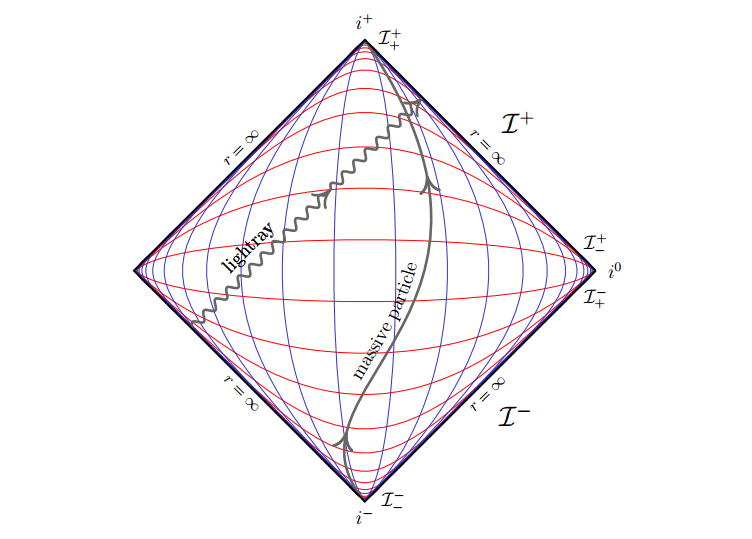
\includegraphics[scale = 0.3]{Penrose-Minkowski.png}
        \end{center}
        vediamo quindi che la geodetica nulla (lightray) ha due estremi in \(\mathcal{I}\). 
        \item Anche la terza è ovvia, perchè chiaramente per Minkowski vale \(R_{\mu\nu} = 0\) in ogni punto.
    \end{enumerate}
}

Ora che abbiamo chiaro cosa significa per uno spaziotempo essere asintodicamente semplice, possiamo enunciare un teorema che ne elenca le principali caratteristiche: 

\thm{Proprietà degli spaziotempi asindoticamente semplici}{

    Sia \(M\) asindoticamente semplice e vuoto, in \(d=4\). Allora valgono le seguenti proprietà: 

    \begin{enumerate}
        \item Ogni geodetica nulla in \(M\) ha un parametro affine illimitato, e \(\mathcal{I} = \mathcal{I}^+ + \mathcal{I}^{-}\), dove \(\mathcal{I}^{\pm}\) è un ipersuperficie nulla, convessa, con topologia \(\mathbb{R} \times S^2\). Sono chiamati infinito futuro/passato nullo. 
        \item \((M, g)\) è globalmente \emph{iperbolico}. Questo vuol dire che possiede una superficie \(\Sigma\) (detta superficie di Cauchy), t.c. \(D(\Sigma) = M\), dove \(D(\Sigma) = D^+(\Sigma) \cup D^-(\Sigma)\), con 
        \begin{align}
            D^+(\Sigma) = p \in M | &\text{ esiste una curva causale inestendibile nel passato} \\ &\text{ passante per p, che interseca } \Sigma
        \end{align}
        \item \(g\) approssima la metrica piatta di Minkowski, vicino ad \(\mathcal{I}\). Dunque, all'infinito nullo lo spazio è piatto.
    \end{enumerate}

}

\pf{}{

Per una prova completa, si veda Hawking, Hellis.

Qui dimostriamo solamente la prima proprietà. Un parametro affine \(\lambda\) nella metrica \(g\) è legato ad un parametro affine nella metrica \(\tilde{g}\), tramite la relazione 

\begin{align}
    \frac{d\lambda}{d\tilde{\lambda}} = \Omega^{-2}
\end{align}

Questa relazione si ottiene direttamente calcolando i simboli di Christoffel. Poichè su \(\mathcal{I} \, \Omega =0\), si ha che l'integrale diverge e \(\lambda\)  è illimitato. 

}


Ora, certamente per queste proprietà l'essere asindoticamente semplici offre dei buoni benefici. D'altra parte, poiché ogni geodetica nulla che parte dall'infinito passato nullo raggiunge l'infinito futuro nullo, a questa categoria non può appartenere nessun bubo nero, se diamo una definizione sensata di buco nero. Infatti, ci aspettiamo che dato un collasso gravitazionale ed una singolarità di curvatura, esiste una regione in cui le geodetiche hanno un parametro affine finito, e finiscono all'interno della singolarità, non in \(\mathcal{I}\). \\

Abbiamo allora bisogno di introdurre una condizione più debole: si dice che uno spazio è \emph{debolmente asindoticamente piatto} se esiste un intorno aperto \(U\) di \(\mathcal{I}\), isometrico ad un intorno aperto di \(\mathcal{I}'\), che è il bordo di \(M'\), uno spaziotempo asindoticamente semplice e vuoto. \\

\nt{In uno spaziotempo asindoticamente semplice e vuoto, avevamo la comoda proprietà che esisteva una superficie di Cauchy. Ragioniamo ora se questa proprietà può essere estesa ad un buco nero. Daremo dopo una definizione precisa di buco nero, ma è chiaro che se questa definizione è sensata, allora le geodetiche che entrano nel buco nero non possono uscirci, e può essere che non esista \(\Sigma\) t.c. \(D(\Sigma) = M\). D'altra parte, uno può chidersi se esiste una superficie parziale \(\Sigma\), tale per cui l'infito futuro nullo sia contenuto nel future domain di \(\Sigma\). Questa osservazione dà luogo alla definizione di spaziotempo predicibile nel futuro.}

\dfn{Predicibilità asindotica nel futuro}{

    Uno spaziotempo asindoticamente semplice e vuoto viene chiamato asindoticamente predicibile nel futuro, se esiste una superficie di Cauchy parziale, tale che \(\mathcal{I}^+ \subset \bar{D^+(\Sigma)}\). 
}

Un esempio di spaziotempo asindoticamente predicibile nel futuro è lo Swartschild. Vedremo più avanti uno spaziotempo che non è asindoticamente predicibile nel futuro. 

Siamo finalmente pronti a dare la definizione di buco nero: 

\dfn{Buco nero}{

    Uno spaziotempo \(M\) si dice contenere un buco nero, se

    \begin{align}
        B := M \setminus J^-(\mathcal{I}^+) \neq \emptyset
    \end{align}

    In particolare, \(B \subset M\) è detta regione del buco nero, ed il bordo \(H\) di \(J^-(\mathcal{I}^+)\) è detto \emph{orizzonte degli eventi}.  
}

\section{Soluzione di Swartschild, orizzonti di Killing, gravità superficiale e temperatura di Hawking}

La più famosa soluzione delle equazioni di Einstein che contiene un buco nero è lo spaziotempo di Swartschild, con metrica 

\begin{align}
    ds^2 = -\left(1-\frac{2m}{r} \right)dt^2 + \frac{dr^2}{\left(1-\frac{2m}{r} \right)} + r^2d\Omega^2
\end{align}

Con alcuni cambiamenti di coordinate si rimuove la singolarità all'orizzonte degli eventi, 

\begin{align}
    ds^2 = -\frac{32 m^2}{r}e^{-r/2m}dU dV
\end{align}

possiamo fare un altro cambiamento di coordinate, passando a delle coordinate compatte: scriviamo 

\begin{align}
    \begin{cases}
        U = \tan\left(\frac{\eta -\zeta}{2} \right) \\
        V = \tan \left(\frac{\eta + \zeta}{2} \right)
    \end{cases}
    \implies ds^2 = \frac{32m^2}{r(\eta, \zeta)}\frac{e^{-r/2m}}{4\cos^2((\eta+\zeta)/2)\cos^2((\eta-\zeta)/2)}(-d\eta^2 + d\zeta^2)
\end{align}

Poiché \(r>0\) (non posso mai andare oltre la singolarità di curvatura), abbiamo trovato che lo spaziotempo di Kruskal è conforme a Minkowski. Da queste considerazioni si determina il diagramma di Penrose dello spaziotempo di Swartschild: 

\begin{center}
    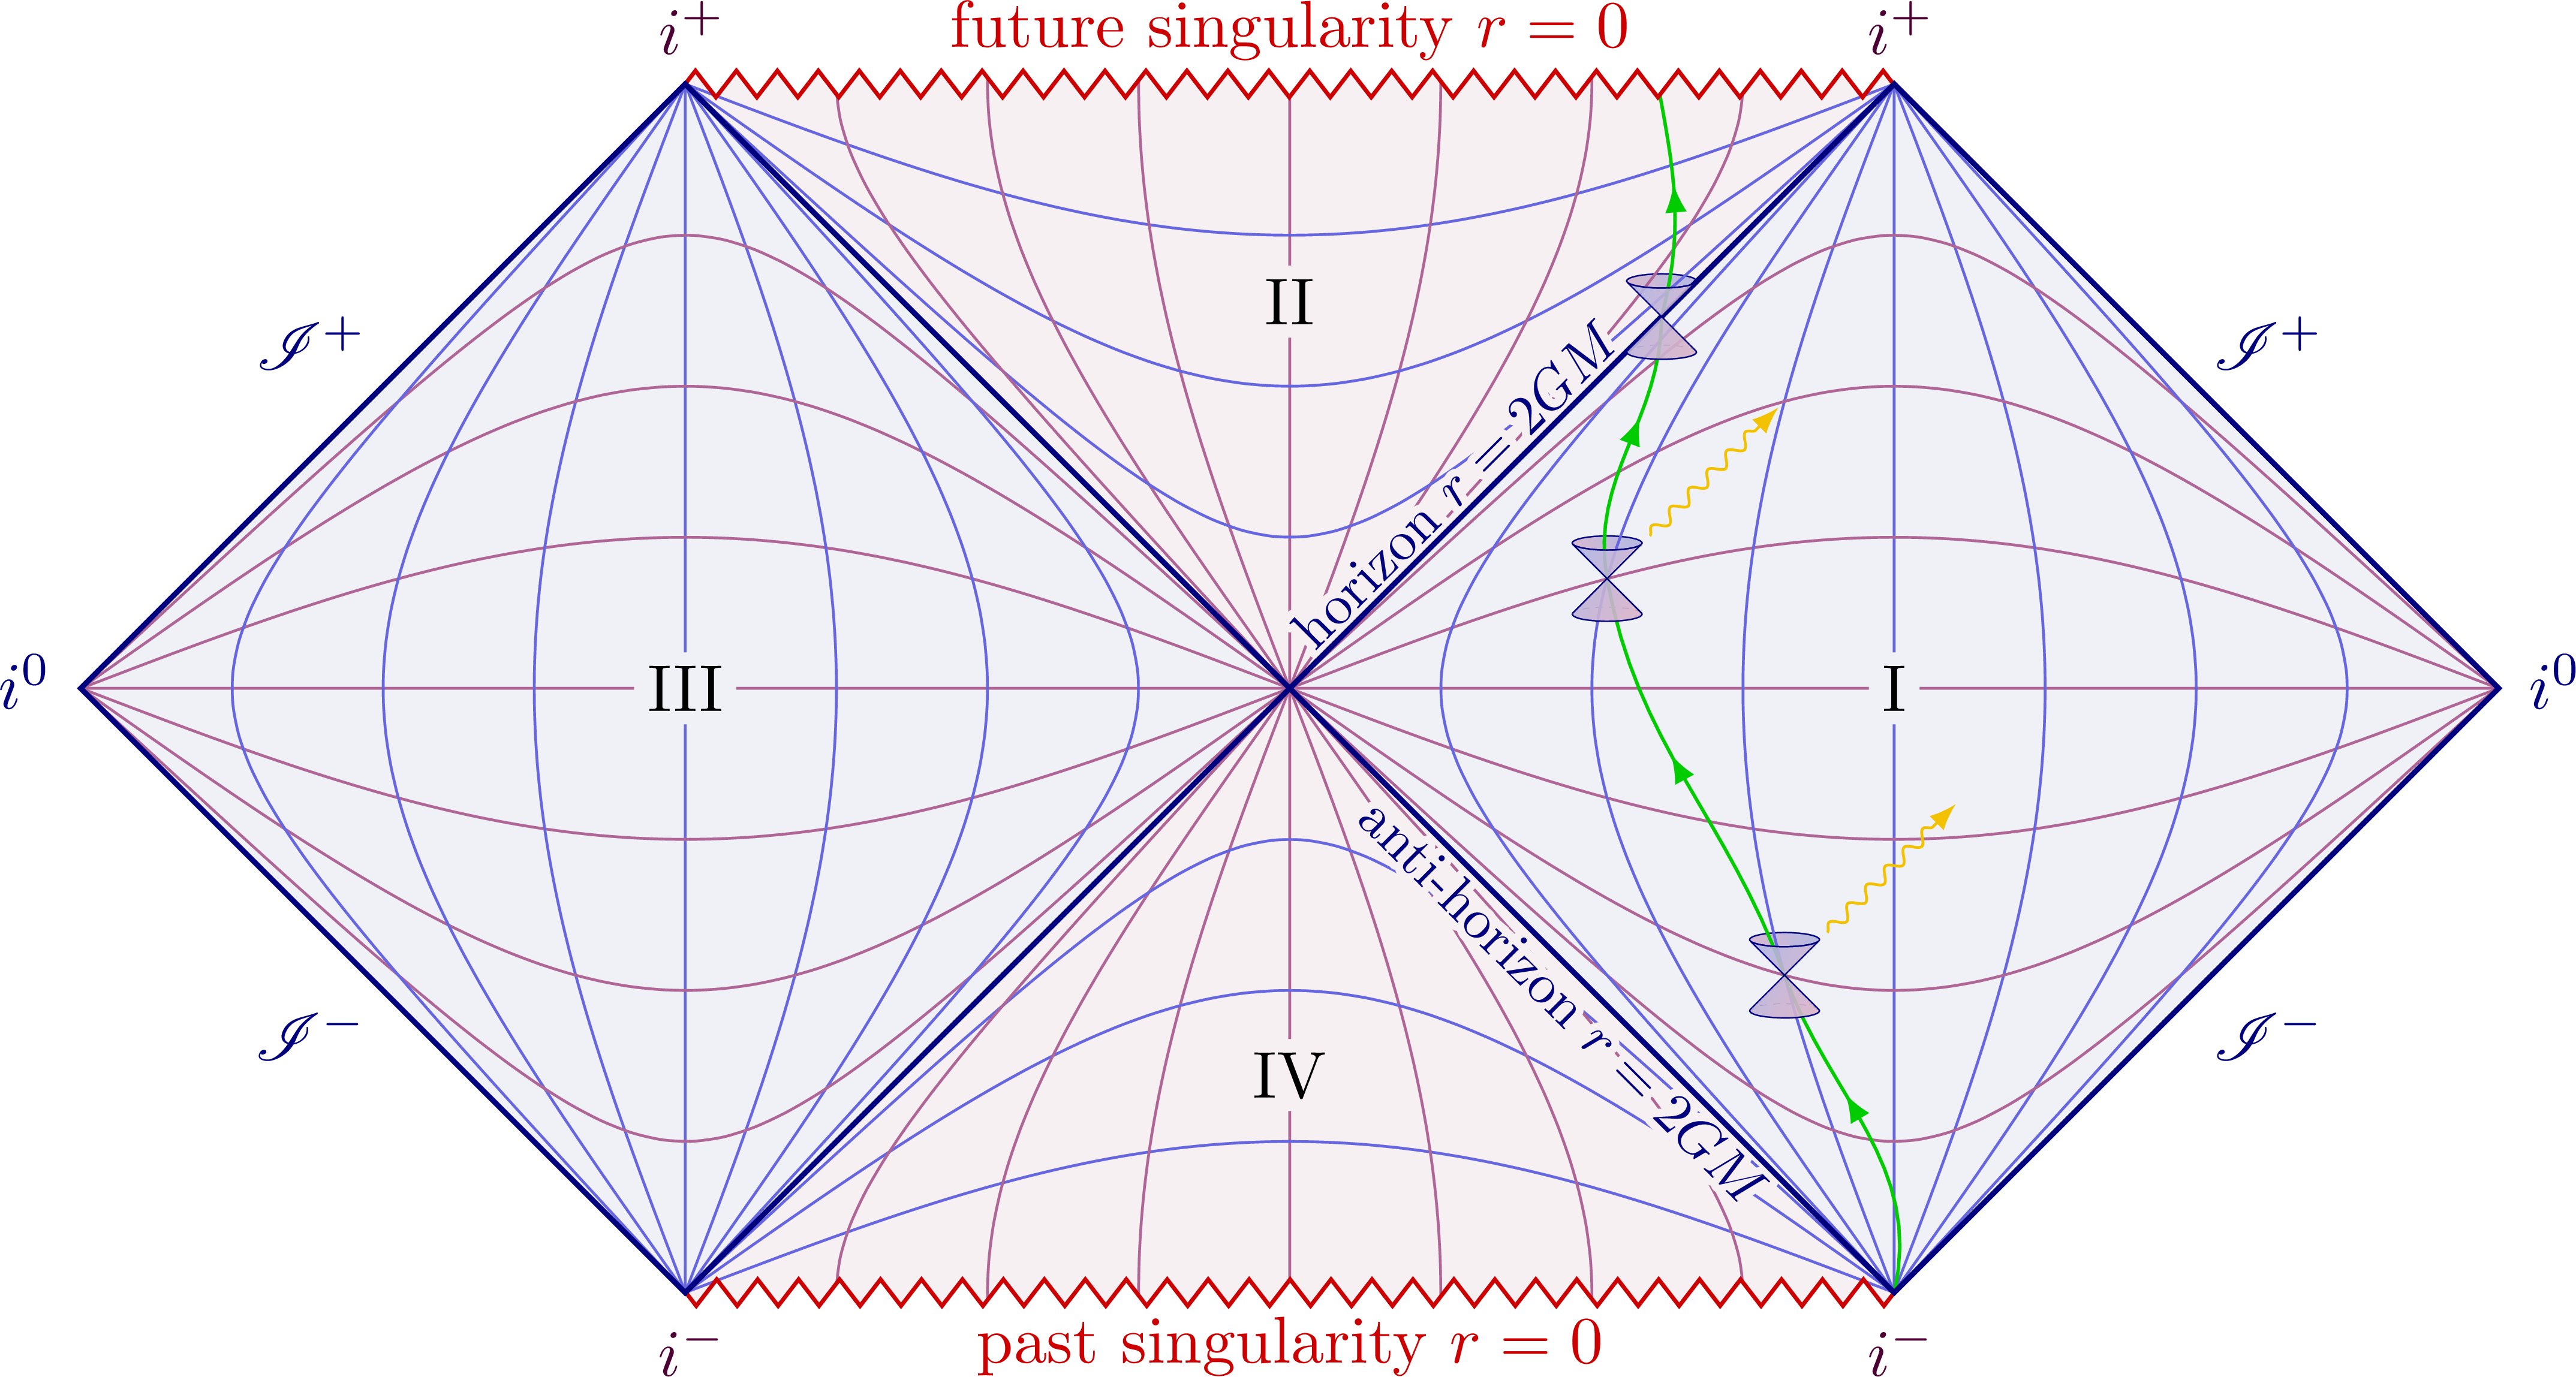
\includegraphics[scale=0.07]{Penrose-Swarzschild.png}
\end{center}

Nota che ogni punto in questo diagramma è una \(S^2\). Dal disegno è immediatamente chiaro che: 

\begin{enumerate}
    \item Il passato causale \(J^-(\mathcal{I}^+)\) è chiaramente l'unione delle regioni I, II, III. 
    \item Il buco nero B, secondo la definizione data sopra, è II. Lo spaziotempo non è asindoticamente semplice e vuoto.
    \item Possiamo facilmente trovare una ipersuperficie tale che nel suo future domain sia contenuto tutto l'infinito futuro nullo. Dunque lo Swartschild è asindoticamente predicibile nel futuro. 
\end{enumerate}

Consideriamo ora la soluzione di Swartschild, se vale \(m<0\). Questa è ancora una soluzione delle equazioni di Einstein, che non ha però un particolare senso fisico. Per noi però è interessante, perché osserveremo per la prima volta una singolarità \emph{nuda}, ed è inoltre un esempio di spaziotempo non predicibile asindoticamente nel futuro. \\

Una comodità di questo spaziotempo è che la singolarità delle coordinate (in \(r = 2m\)) è oltre la singolarità di curvatura (in \(r=0\)), e non abbiamo bisogno allora di passare alle coordinate di Kruskal. Semplicemente allora definiamo 

\begin{align}
    r_* = \int \frac{dr}{1-2m/r} = r +2m\ln\biggr|\frac{2m}{r}-1 \biggr|
\end{align}

In questo modo, \(\frac{dr}{dr_*} = 1 - \frac{2m}{r}\), e quindi se passo da \(r \rightarrow r_*\) la metrica diventa 

\begin{align}
    ds^2 = \left(1-\frac{2m}{r} \right)(-dt^2 + dr_*^2)
\end{align}

trascurando per il momento la parte angolare. Allora, posso poi considerare un altro cambio di coordinate, 
 
\begin{align}
    \begin{cases}
        u = t -r_* \\ v = t+ r_*
    \end{cases}
    \implies ds^2 = -\left(1 - \frac{2m}{r} \right)dudv
\end{align}

per compattificare prendiamo al solito 

\begin{align}
    \begin{cases}
        u = \tan(u'/2) \\ v = \tan(v'/2)
    \end{cases}
    \implies ds^2 = -\left(1 - \frac{2m}{r} \right)\frac{1}{4\cos^2(u'/2)\cos^2(v'/2)}du'dv'
\end{align}

Si disegna allora il diagramma di Penrose: 

\begin{multicols}{2}
    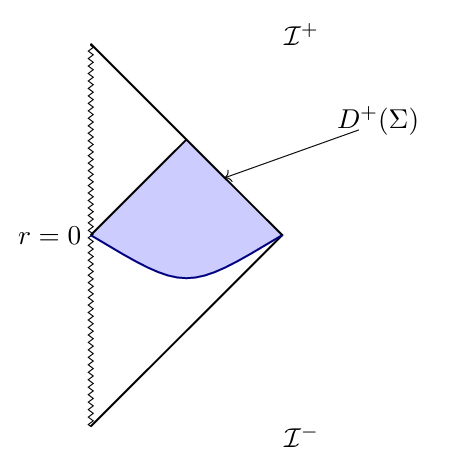
\includegraphics[scale = 0.4]{Penrose-naked.singularity.png}

    \columnbreak

    Osserviamo che non è predicibile asindoticamente nel futuro, e che esistono geodetiche che partono dalla singolarità ed arrivano all'infinito futuro nullo. In questi casi si parla di singolarità nuda, perché non si è "vestita" con un orizzonte degli eventi.

\end{multicols}

Nel teorema che introduceva le proprietà di uno spaziotempo asindoticamente semplice e vuoto, abbiamo parlato di ipersuperficie nulla, senza però definirla. Vediamo ora una sua definizione rigorosa: 

\dfn{Ipersuperficie nulla}{

    Sia \(S(x)\) una funzione liscia delle coordinate. Consideriamo una famiglia di ipersuperfici \(S = cost.\). Allora, i campi vettoriali normali alla superficie sono dati da 

    \begin{align}
        \ell = \tilde{f}(x)g^{\mu\nu}(\partial_\nu S)\partial_\mu
    \end{align}

    con \(\tilde{f}(x)\) una funzione arbitraria delle coordinate non-nulla. Se vale \(\ell^2 = 0\) per una ipersuperficie \(N\) appartenente alla famiglia, questa è detta \emph{ipersuperficie nulla}. 
}

Le ipersuperfici nulle godono di alcune proprietà. Ad esempio, sia \(N\) un'ipersuperficie nulla, con \(\ell\) vettore normale. Dato invece \(t\) un vettore tangente, vale \(<\ell, t> =0\). Ma siccome \(<\ell, \ell> =0\), segue che anche \(\ell\) è un vettore tangente, cioè possiamo scrivere 

\begin{align}
    \ell^\mu = \frac{dx^\mu}{d\lambda}
\end{align}

\clm{}{}{
    Le curve integrali \(x^\mu(\lambda)\), cioè che soddisfano 
    \begin{align}
        \ell^\mu = \frac{dx^\mu}{d\lambda}
    \end{align}
    sono geodetiche. 
}

\pf{}{
    Dalla definizione di ip. nulla, sappiamo che il vettore normale è dato da 
    \begin{align}
        \ell^\mu = \tilde{f}(x)g^{\mu\nu}(\partial_\nu S)
    \end{align}

    le curve integrali sono geodetiche se \(\nabla_\ell \ell^\mu \propto \ell^\mu\). Calcoliamo, allora: 

    \begin{align}
        \ell_\rho \nabla^\rho (\tilde{f}g^{\mu\nu}(\partial_\nu S))
    \end{align}

    Inanzitutto svolgiamo la derivata del prodotto: 

    \begin{align}
        \ell_\rho (\partial^\rho\tilde{f})g^{\mu\nu}\partial_\nu S + \ell_\rho \tilde{f}g^{\mu\nu}\nabla^\rho\partial_\nu S
    \end{align}

    ora possiamo sostituire \(g^{\mu\nu}\partial_\nu S = \ell^\mu \tilde{f}\), e ricordo anche che per uno spazio a torsione nulla, vale \(\nabla^\rho\partial_\nu S = \nabla_\nu \partial^\rho S\). Scriviamo allora 

    \begin{align}
        \nabla_\ell \ell^\mu = \ell_\rho (\partial^\rho \ln \tilde{f})\ell^\mu + \tilde{f}\ell^\rho \nabla^\mu (\partial_\rho S)
    \end{align}

    Se poi \(\ell^\rho = \frac{dx^\rho}{d\lambda}\), vale 
    
    \begin{align}
        \nabla_\ell \ell^\mu &= \ell^\mu \frac{d\ln \tilde{f}}{d\lambda} + \tilde{f}\ell^{\rho}\nabla^\mu(\tilde{f}^{-1}\ell_\rho) \\
        &= \ell^\mu \frac{d\ln \tilde{f}}{d\lambda} + \ell^{\rho}\nabla^\mu(\ell_\rho) + \ell^2 (\partial^\mu \ln\tilde{f})
    \end{align}

    Ora, a questo punto se valuto l'espressione su \(N\), l'ultimo pezzo è nullo perché \(\ell^2 = 0\). Il primo pezzo è già a posto, perché voglio dimostrare \(\nabla_\ell \ell^\mu \propto \ell^\mu\). Mi manca allora da gestire quello in mezzo, che posso riscrivere come \(\frac{1}{2}\partial^\mu \ell^2\). Il fatto che \(\ell^2 = 0\) su \(N\), non vuol dire che \(\partial^\mu\ell^2 =0\). D'altra parte, vuol dire che come vettore è ortogonale a tutti i vettori tangenti di N, cioè 

    \begin{align}
        \phi_\mu (\partial^\mu \ell^2) = 0 
    \end{align}

    questo basta a mostrare che è proporzionale alla normale \(\ell^\mu\), ed dunque le curve sono geodetiche. Una parametrizzazione affine è possibile scegliendo in modo adatto \(\tilde{f}\). 
}

Le geodetiche di questo tipo \emph{nulle}, sono detti \emph{generatori nulli} di \(N\). 

\ex{Superfici nulle nello spazio di Kruskal}{
    Prendi lo spaziotempo di Kruskal. Come famiglia di ipersuperfici, prendi quelle dove \(U = \) cost. Allora una superficie nulla è data da \(N = \left\{U = 0 \right\}\). Infatti, il vettore normale è allora dato da 

    \begin{align}
        \ell &= \tilde{f}g^{\mu\nu}\partial_\nu U \partial_\mu
    \end{align}

    ma \(\partial_\nu U = \delta_\nu^U\), e dalla forma della metrica si ottiene 

    \begin{align}
        \ell = \tilde{f}g^{UV}\partial_V = -\frac{\tilde{f}r}{16m^3}e^{r/2m}\partial_V
    \end{align}

    Calcoliamo allora 

    \begin{align}
        \ell|_{U=0} = -\frac{\tilde{f}e}{8m^2}\partial_V \implies \ell^2|_{N} = 0
    \end{align}

    Perché dalla forma della metrica è evidente che \(<\partial_V, \partial_V> =0\). In questo caso in realtà \(\ell^2 = 0\) ovunque, e \(\partial^\mu \ell^2 =0\). Dunque la parametrizzazione affine si recupera se \(\tilde{f} = \) cost. , ad esempio in modo tale che \(\ell = \partial_V\). Dunque, abbiamo mostrato che \(V\) è un parametro affine per i generatori di ipersuperfici nulle.  
}

\dfn{Orizzonti di Killing}{

    Sia \(N\) ipersuperficie nulla. Se esiste un campo vettoriale di Killing \(\xi\) \emph{normale} ad \(N\), si dice che l'ipersuperficie è un'orizzonte di Killing. 
}

Sia allora \(\ell\) la normale di \(N\), con parametrizzazione affine (i.e. \(\nabla_\ell \ell = 0\)). Siccome \(\xi = f\ell\) su \(N\) (essendo anche lui normale ad \(N\), deve essere sempre parallelo alla normale \(\ell\)), vale che 

\begin{align}
    \nabla_\xi \xi &= \nabla_{f\ell}(f\ell) = f \nabla_{\ell}(f\ell) \\
    &= f[(\partial_\ell f)\ell + f\partial_\ell \ell] \\
    &= \underbrace{f \ell}_{=\xi} \underbrace{(\ell^\mu \partial_\mu f)}_{ =: \mathcal{H}}
\end{align}

La funzione \(\mathcal{H} = \ell^\mu \partial_\mu f\) è di grande importanza, ed è detta \emph{gravità superficiale}. Questa dipende solo da \(\xi\), e deriviamo adesso una formula che permette di calcolarla rapidamente: 

Il teorema di Frobenius dice che, siccome \(\xi\) è normale ad \(N\), vale 

\begin{align}
    \xi_{[\mu}\nabla_\nu \xi_{\rho]} = 0
\end{align}

Unito alla proprietà dei vettori di Killing, \(\nabla_\mu\xi_\nu = -\nabla_\nu\xi_\mu\), otteniamo 

\begin{align}
    \xi_\rho\nabla_\mu\xi_\nu + \xi_\nu\nabla_\rho\xi_\mu + \xi_\mu\nabla_\nu\xi_\rho = 0
\end{align}

oppure 

\begin{align}
    \xi_\rho \nabla_\mu\xi_\nu = \xi_\nu\nabla_\mu\xi_\rho - \xi_\mu\nabla_\nu \xi_\rho
\end{align}

per far "saltare fuori" la gravità superficiale, ho bisogno di fattori \(\nabla_\xi \xi = \xi^\mu \nabla_\mu \xi\). Per farlo, contraggo l'espressione con \(\nabla^\mu\xi^\nu\): 

\begin{align}
    \xi_\rho (\nabla_\mu\xi_\nu)(\nabla^\mu\xi^\nu) = (\nabla^\mu \xi^\nu)\xi_\nu \nabla_\mu \xi_\rho -  (\nabla^\mu\xi^\nu)\xi_\mu\nabla_\nu \xi_\rho
\end{align}

Mi accorgo però che 

\begin{align}
    (\nabla^\mu\xi^\nu)\xi_\nu \nabla_\mu \xi_\rho = (\nabla^\nu\xi^\mu)\xi_\mu \nabla_\nu \xi_\rho = - (\nabla^\mu\xi^\nu)\xi_\mu \nabla_\nu \xi_\rho
\end{align}

D'ora in poi valuto tutte le espressioni sulla ipersuperficie nulla, dove vale \(\nabla_\xi \xi^\mu = \mathcal{H}\xi^\mu\).  Ottengo:  

\begin{align}
    \xi_{\rho}(\nabla_\mu \xi_\nu)(\nabla^\mu \xi^\nu) &= -2 (\nabla^\mu \xi^\nu)\xi_\mu \nabla_\nu \xi_\rho \\
    &= -2\mathcal{H}\xi^\nu\nabla_\nu \xi_\rho \\
    &= -2\mathcal{H}^2 \xi_\rho 
\end{align}

Abbiamo scoperto che vale 

\begin{align}
    \mathcal{H}^2 = -\frac{1}{2}(\nabla_\mu\xi_\nu)(\nabla^\mu\xi^\nu)|_{N}
\end{align}

La gravità superficiale ha molte proprietà utili. Scopriremo più avanti che è legata alla temperatura del buco nero. D'altra parte, vale anche 

\mlemma{}{
  Sulle orbite di \(\xi\), \(\mathcal{H}\) è costante 
}
  

\pf{}{
    La dimostrazione di questo usa il Killing-vector-lemma, ovvero la nota relazione 

    \begin{align}
        \nabla_\rho \nabla_\mu \xi^\nu = R^\nu_{\mu\rho\sigma}\xi^\sigma
    \end{align}

    Ora, sia \(t\) vettore tangente di \(N\). Dalla formula precedente, calcolo che 

    \begin{align}
        \nabla_t \mathcal{H}^2 &= -(\nabla^\mu\xi^\nu)\nabla_t(\nabla_\mu\xi_\nu) \\
        &= -(\nabla^\mu\xi^\nu)t^\rho (\nabla_\rho\nabla_\mu \xi_\nu) \\
        &= -(\nabla^\mu\xi^\nu)t^{\rho}R_{\mu\nu\rho\sigma}\xi^{\sigma}
    \end{align}

    Poiché \(\xi\) è anche tangente (ricorda che \(xi \propto \ell\), e \(\ell^2|_N = 0\)), vale quindi che 

    \begin{align}
        \nabla_\xi \mathcal{H}^2 = - (\nabla^\mu\xi^\nu)R_{\mu\nu\rho\sigma}\xi^\rho\xi^\sigma = 0 
    \end{align}

    perché ricorda che il Riemann è antisimmetrico nello scambio \(\rho \leftrightarrow \sigma\). 
}

Ora, sia \(\mathcal{H} \neq 0\) su un orbita di \(\xi\), in \(N\). Questa orbita coincide con solo una parte di un generatore nullo di \(N\). Per vedere questo, scegli delle coordinate su \(N\), t.c. \(\xi = \partial_\alpha\). Se \(\alpha(\lambda)\) è un'orbita di \(\xi\), con parametro affine \(\lambda\), si ha che 

\begin{align}
    \xi|_{\text{orbita}} = \frac{d\lambda}{d\alpha}\frac{d}{d\lambda} = f\ell
\end{align}

se scegliamo \(f = \frac{d\lambda}{d\alpha}\), allora vale 

\begin{align}
    \ell = \frac{d}{d\lambda} = \frac{dx^\mu}{d\lambda}\partial_\mu
\end{align}

La gravità superficiale si può scrivere come 

\begin{align}
    \mathcal{H} = \xi^\mu \partial_\mu \ln \abs{f}
\end{align}

cioè, in questo caso, 

\begin{align}
    \mathcal{H} = \frac{\partial}{\partial \alpha}\ln \abs{f}
\end{align}

posso integrare allora rispetto ad \(\alpha\), e ottenere (siccome \(\mathcal{H}\) è costante)

\begin{align}
    f = f_0 e^{\mathcal{H}\alpha}
\end{align}

La costante \(f_0\) è una costante di integrazione. Siccome possiamo sempre fare una traslazione di \(\alpha\) a piacere, possiamo prendere \(f_0 = \pm\mathcal{H}\). 

Allora, 

\begin{align}
    f = \frac{d\lambda}{d\alpha} = \pm\mathcal{H}e^{\mathcal{H}\alpha} \implies \lambda = \pm e^{\mathcal{H}\alpha} + c 
\end{align}

dunque, per \(\alpha \in (-\infty, +\infty)\), copriamo le parti \(\lambda > 0\) e \(\lambda <0\) del generatore di \(N\). Il punto invece \(\lambda =0\) è un punto di biforcazione, ed è detto punto fisso di \(\xi\). Si può far vedere che questo punto è una 2-sfera, detta 2-sfera di biforcazione. 

\ex{2-sfera di biforcazione in spaziotempo di Kruskal}{

    Considera \(N = \left\{U=0 \right\} \cap \left\{V=0 \right\}\). Lo spaziotempo di Kruskal è statico, ed in particolare \(\xi = \partial_t\) è killing. Esplicitamente, il vettore in termini delle coordinate che entrano nella metrica sono date da 

    \begin{align}
        \xi = \partial_t = \frac{1}{4m}(V\partial_V - U\partial_U)
    \end{align}

    in particolare, 

    \begin{align}
        \xi = \begin{cases}
            \frac{1}{4m}(V\partial_V), \, U=0 \\
            -\frac{1}{4m}(U\partial_U), \, V=0
        \end{cases} = f\ell
    \end{align}

    cioè 

    \begin{align}
        f = \begin{cases}
            \frac{V}{4m} \\
            -\frac{U}{4m}
        \end{cases} \quad \ell = \begin{cases}
            \partial_V \\ \partial_U
        \end{cases}
    \end{align}

    Inanzitutto, notiamo che \(\ell\) è normale ad entrambi le ipersuperfici, dunque anche \(\xi\) lo è. Segue in paricolare che \(N\) è un orizzonte di Killing. 

    Calcoliamo la gravità superficiale: 

    \begin{align}
        \mathcal{H} = \xi^\mu\partial_\mu \ln \abs{f} = \begin{cases}
            \frac{U}{4m}\partial_U \ln \abs{U} = \frac{1}{4m} \\
            -\frac{V}{4m}\partial_V \ln \abs{V} = -\frac{1}{4m}
        \end{cases}
    \end{align}
}

\ex{Ipersuperfici nulle e orizzonti di Killing in Kruskal}{

    Ricordiamo la metrica di Kruskal: 

    \begin{align}
        ds^2 = \frac{32m^2}{r}e^{2m/r}dU dV
    \end{align}

    Sappiamo (spaziotempo statico), che \(\xi = \partial_t\) è Killing. Nelle coordinate di Kruskal, vale \(\xi = \frac{1}{4m}(U\partial_U - V\partial_V)\). Ora, cominciamo a considerare la ipersuperficie \(\mathcal{N}_1\) def. da \(U = 0\). Si ha allora che \(\xi|_{\mathcal{N}_1} = -\frac{V}{4m}\partial_V\). Calcolo la normale alla ipersuperficie: 

    \begin{align}
        \ell|_{\mathcal{N}_1} = \tilde{f}g^{\mu\nu}(\partial_\nu U)\partial_\mu
    \end{align}

    Chiaramente, \(\partial_\nu U \neq 0\) s.se \(\nu = U\), quindi 

    \begin{align}
        \ell|_{\mathcal{N}_1} = \tilde{f}g^{\mu V}\partial_\mu = \tilde{f}g^{U V}\partial_V
    \end{align}

    Dove l'ultimo passaggio segue dalla forma della metrica. Posso scegliere allora \(\tilde{f}\) in modo tale che valga \(\ell_{\mathcal{N}_1} = \partial_V\). Questa scelta corrisponde alla parametrizzazione affine. Infatti, calcolo 

    \begin{align}
        \nabla_\ell \ell^\mu = \ell^\rho (\partial_\rho \ell^\mu + \Gamma^\mu_{\alpha \rho}\ell^{\alpha})
    \end{align}

    L'unica componente non nulla di \(\ell\) è \(\ell^V = 1\) che è chiaramente costante. Si ha allora 

    \begin{align}
        \nabla_\ell \ell^\mu = \Gamma^\mu_{VV}
    \end{align}

    Poiché però \(g_{VV} =0\), e su \(\mathcal{N}_1\) \(\partial_V\) è Killing, segue che \(\nabla_\ell \ell^\mu = 0\). 
    
    Segue allora che \(\mathcal{N}_1\) è un orizzonte di Killing. Se voglio poi trovare la gravità superficiale, scrivo 

    \begin{align}
        \xi = f\ell \implies f = -\frac{1}{4m}
    \end{align}

    A questo punto vale la formula 

    \begin{align}
        \kappa = \xi^\rho \partial_\rho \ln f = -\frac{V}{4m}\partial_V \ln(V) = -\frac{1}{4m}
    \end{align}
}

\ex{Calcolo della gravità superficiale con formula alternativa}{

    Possiamo controllare che la formula che abbiamo trovato per la gravità superficiale, 

    \begin{align}
        \kappa^ 2 = -\frac{1}{2}(\nabla_\mu \xi_\nu)(\nabla^\mu \xi^\nu)|_{\mathcal{N}}
    \end{align}

    Dia lo stesso risultato della formula "diretta", \(\kappa = \ell^\rho \partial_\rho f\). In questo caso la prima era immediata e la seconda impiega un po di lavoro, ma il calcolo èì istruttivo ed è un semplice risultato di applicazione delle regole delle derivate covarianti. Considera \(\xi\) non per forza in \(\mathcal{N}\): allora vale 

    \begin{align}
        \xi^U = \frac{U}{4m}, \quad \xi^V = -\frac{V}{4m}
    \end{align}

    per comodità future, calcoliamo il vettore contravariante. Abbassando gli indici con la metrica troviamo 

    \begin{align}
        \xi_U = g_{UV}\xi^V = \frac{4m^2 V}{r}e^{-r/2m}, \quad \xi_V = g_{VU}\xi^U = -\frac{4m^2 U}{r}e^{-r/2m}
    \end{align}

    Devo calcolare le componenti del tensore \(2 \times 2\) \(\nabla_\mu \xi_\nu\). Essendo antisimmetrico, ha solo un parametro libero, dato da 

    \begin{align}
        \nabla_U \xi_V = \partial_U \xi_V - \Gamma_{\rho U V}\xi^\rho = \partial_U \xi_V - \Gamma_{VUV}\xi^V - \Gamma_{UUV}\xi^U
    \end{align}

    Ma i simboli di Christoffel \(\Gamma_{VUV}, \, \Gamma_{UUV}\) sono identicamente nulli ovunque, data la forma della metrica. Segue che 

    \begin{align}
        \nabla_U \xi_V = -\frac{4m^2}{r}e^{-r/2m} + \frac{4m^2 U}{r^2}e^{-r/2m} + \frac{2m U}{r^2}e^{-r/2m} \implies \nabla_U \xi_V |_{\mathcal{N}} = -\frac{2m}{e}
    \end{align}

    Calcoliamo allora 

    \begin{align}
        (\nabla_\nu \xi_\mu)(\nabla_\alpha \xi_\beta)g^{\nu\alpha}g^{\mu\beta} &= 2(\nabla_V \xi_U)(g^{UV})^2(\nabla_V \xi_U) \\
        &= -\frac{8m^2}{e^2}(g^{UV})^2 \\
        &= -\frac{1}{8m^2}
    \end{align}

    Cioè si ottiene 

    \begin{align}
        \kappa^2 = \frac{1}{16m^2}
    \end{align}

    come ci aspettavamo. 


}

In precedenza, abbiamo detto che la gravità superficiale è legata alla temperatura del buco nero. Indaghiamo insieme ora questa relazione. In particolare, è possibile studiare teorie di campi nello spaziotempo di buconero, usando gli integrali di cammino euclideo. In Minkowski, questo vuol dire fare la continuazione analitica (anche detta \emph{rotazione di Wick}) \(t \rightarrow -i\tau\). Ad esempio, possiamo vedere come è fatta la metrica euclidea di Swartschild: 

\begin{align}
    ds^2_E = \left(1-\frac{2m}{r} \right)d\tau^2 + \frac{dr^2}{\left(1-\frac{2m}{r} \right)} + r^2d\Omega^2
\end{align}

Similmente alla sua controparte Lorentziana, la metrica è singolare per \(r = 2m\). Per indagare allora le proprietà della metrica vicino alla singolarità, esattamente come si fa in metrica lorentziana, eseguiamo la sostituzione: 

\begin{align}
    r -2m = \frac{x^2}{8m} \implies 1 - \frac{2m}{r} = \frac{r-2m}{r} = \frac{x^2}{8m(2m+x^2/8m)} = \frac{x^2}{16m^2} + o(x^4)
\end{align}

Inoltre, \(dr = \frac{2xdx}{8m} = \frac{xdx}{4m}\), così che la metrica nella nuova coordinata si scrive 

\begin{align}
    ds^2_E = (x\mathcal{H})^2d\tau^2 + dx^2 + 4m^2d\Omega^2
\end{align}

Osserviamo bene questa metrica: la seconda parte è semplicemente la metrica standard sulla \(S^2_{2m}\). Invece, la prima ricorda molto la metrica sul piano euclideo, in coordinate polari: 

\begin{align}
    ds^2_{\mathbb{E}^2} = dr^2 + r^2 d\theta^2, \quad r \in \mathbb{R}, \, \theta \in [-\pi, \pi]
\end{align}

l'unica differenza è dunque che \(\theta\) è una coordinata compatta. Una analisi più profonda mostra che se la metrica non è euclidea, presenta una singolarità conica. Questo porta ad identificare 

\begin{align}
    \tau \simeq \tau + \frac{2\pi}{\mathcal{H}}
\end{align}

Il periodo del tempo immaginario è legato alla temperatura. Infatti, nell'approccio path-integral della teoria dei campi, si esprime l'elemento di matrice per andare da uno stato iniziale al tempo \(t_1\) ad uno stato finale al tempo \(t_2\) secondo: 

\begin{align}
    \Braket{\phi_1, t_1 | \phi_2, t_2} = \int [D\phi]e^{\frac{i S(\phi)}{\hbar}}
\end{align}

dove \(S\) è l'azione. Il path-integral va preso su tutte le configurazioni dei campi \(\phi\), che prendono valori \(\phi_1\) al tempo \(t_1\), e \(\phi_2\) al tempo \(t_2\). D'altra parte l'elemento di matrice lo si può anche esprimere attraverso l'operatore di evoluzione temporale: 

\begin{align}
    \bra{\phi_2}e^{-\frac{i}{\hbar}H(t_2-t_1)}\ket{\phi_1}
\end{align}

se prendiamo  \(\phi_1 = \phi_2\), \(t_2 - t_1 = -i\beta\hbar\), e sommiamo su tutti gli \(\phi_1\), si ottiene 

\begin{align}
    \sum_{\phi_1}\bra{\phi_1}e^{-\frac{i}{\hbar}H(-i\beta \hbar)}\ket{\phi_1} = \text{Tr}(e^{-\beta H}) = \int [d\phi]e^{\frac{iS(\phi)}{\hbar}}
\end{align}

La funzione \(Z = \text{Tr}(e^{-\beta H})\) è detta funzione di partizione, che descrive un campo \(\phi\) alla temperatura \(T = (K_B \beta)^{-1}\). Ma \(\beta\) è legato al periodo dei campi! Se il periodo, come nel caso del buco nero di Swartschild, è dato da \(2\pi/\mathcal{H}\), si ottiene 

\begin{align}
    \beta \hbar = \frac{2\pi}{\mathcal{H}} \implies T_H = \frac{\hbar \mathcal{H}}{2\pi K_B}
\end{align}

che è la \emph{temperatura di Hawking} per il buco nero di Swartschild. Nota bene che la temperatura è proporzionale a \(\hbar\) per cui nel limite classico \(\hbar \rightarrow 0\) è nulla! Dunque si tratta di un fenomeno quantistico. 

\section{Buchi neri carichi e rotanti}

\dfn{Spaziotempo assisimmetrico}{
    Uno spaziotempo si dice \emph{assisimmetrico}, se esiste un campo vettoriale di Killing, \(m\), di tipo spazio vicino all'infinito spaziale, tale per cui tutte le sue orbite sono \emph{chiuse}. 

    Si possono scegliere allora delle coordinate tali per cui \(m = \partial_\varphi\), con \(\varphi\) una coordinata tale che \(\varphi \simeq \varphi + 2\pi\)
}

Si ricorda che nel caso di spaziotempo con simmetria sferica, valeva il teorema di Birckhoff, che diceva che ogni spaziotempo nel vuoto, con simmetria sferica, era anche statico. In quel caso allora, l'unica soluzione possibile delle equazioni di Einstein era quella di Swartschild. Per il caso assisimmetrico, esiste un teorema simile: 

\thm{Carten-Robinson}{
    Sia \((M, g)\) uno spaziotempo asindoticamente piatto, stazionario e assisimmetrico, con \(R_{\mu\nu} = 0\), e non singolare su e fuori un orizzonte. 

    Allora \((M, g)\) è un membro della \emph{famiglia di Kerr}, con i due parametri \(M, J\) (massa e momento angolare). 
}

questi due teoremi possono essere generalizzati anche per le equazioni di Einstein-Maxwell, i.e. le equazioni del moto che seguono dall'azione 

\begin{align}
    I = \int d^4x \sqrt{-g}\left[\frac{R}{16\pi G} - \frac{1}{4}F_{\mu\nu}F^{\mu\nu} \right]
\end{align}

ovvero 

\begin{align}
    G_{\mu\nu} = 8\pi G T_{\mu\nu}^{\text{  em}}, \quad \nabla_\mu F^{\mu\nu} = 0 \implies \partial_\mu (\sqrt{-g}F^{\mu\nu}) = 0 
\end{align}

dove il tensore di energia momento è quello elettromagnetico, ovvero 

\begin{align}
    T_{\mu\nu}^{\text{  em}} = F_{\mu\rho}F^\rho_\nu - \frac{1}{4}g_{\mu\nu}F_{\alpha\beta}F^{\alpha\beta}
\end{align}

Il risultato è che i buchi neri asintodicamente piatti e stazionari devono appartenere alla famiglia di \emph{Kerr-Neumann}, a 3 parametri. Nota che non abbiamo dovuto richiedere l'assisimmetria: questa in realtà è sempre verificata per un buco nero stazionario, ed è il risultato di un teorema dovuto a Wald e Hawking. La famiglia di Kerr-Neumann, ha metrica

\begin{align}
    ds^2 = -\frac{(\Delta - a^2\sin^2\theta)}{\rho^2}dt^2 -2a\sin^2\theta \frac{r^2 + \Delta^2 - \Delta}{\rho^2}dtd\varphi + \frac{(r^2 + a^2)-\Delta a \sin^2\theta}{\rho^2}\sin^2\theta d\varphi^2 + \frac{\rho^2}{\Delta}dr^2 + \rho^2d\theta^2
\end{align}

dove \(\rho^2 = r^2 + a^2\cos^2\theta\), e invece \(\Delta = r^2 - 2mr + a^2 +e^2\). I tre parametri sono la massa \(m\), la carica \(e = \sqrt{Q^2 + P^2}\), e il parametro \(a\), che è ad occhio legato alla rotazione (il termine fuori dalla diagonale \(dtd\varphi\) è infatti proporzionale ad \(a\)). In effetti più avanti mostreremo come \(J = ma\), con \(J\) il momento angolare. 

Essendo una soluzione delle equazioni di Einstein-Maxwell, sarebbe incompleta senza la 1-forma di Maxwell: 

\begin{align}
    A = \frac{Qr(dt - a\sin^2\theta d\varphi) - P\cos\theta[adt - (r^2+a^2)d\varphi]}{\rho^2}
\end{align}

in cui riconosciamo un termine di monopolo elettrico, \(\frac{Qr}{\rho^2}dt\), di dipolo elettrico \(\propto \sin^2\theta\) e anche di monopolo magnetico, \(\propto \cos\theta d\varphi\). 

Questo sistema di coordinate \((t, r, \theta, \varphi)\) sono dette coordinate di Boyer-Lindsyt. Valgono in particolare i seguenti limiti: 

\begin{enumerate}
    \item \(a = e = 0 \implies\) buco nero di Swartschild
    \item \(a=0 \implies \) buco nero carico e statico
    \item \(e =0 \implies\) buco nero di Kerr
\end{enumerate}

La soluzione di Kerr è importante dal punto di vista astrofisico, perché rappresenta con buona approssimazione la metrica di una stella rotante a grande distanza, dove tutti i momenti di multipolo, tranne \(\ell = 0, 1\) sono rilevanti. Questa metrica persenta alcune singolarità di coordinate, similmente allo Swartschild, per: 

\begin{enumerate}
    \item \(\theta = 0\), sull'asse di simmetria 
    \item \(\Delta =0\), molto simile allo Swartschild. 
\end{enumerate}

In particolare, possiamo scrivere \(\Delta = (r-r_-)(r+r_+)\), con \(r_\pm = m \pm \sqrt{m^2 -a^2}\). Ci sono allora 3 casi da considerare: 

\begin{enumerate}
    \item \(m^2 < a^2\): in questo caso \(r_\pm\) sono complessi, e quindi \(\Delta\) non si annulla mai. Rimane comunque la singolarità di curvatura, quando \(\rho^2 =0 \implies r=0, \theta = \pi/2\), che si dimostra studiando l'andamento di tensori di curvatura non nulli come \(R_{\mu\nu\rho\sigma}R^{\mu\nu\rho\sigma}\). Per studiare la singolarità, usiamo le coordinate di Kerr-Shild, che rimuovono la singolarità di coordinate in \(\theta = 0\). Queste sono date da 
    \begin{align}
        &x +iy = (r + ia)\sin\theta\exp\left(i\int d\varphi + \frac{a}{\Delta}dr \right) \\
        &z = r\cos\theta \\
        &\tilde{t} = \int \left(dt + \frac{r^2+a^2}{\Delta}dr \right) -r
    \end{align}
    si trova allora che
    \begin{align}
        x^2 + y^2 +z^2 = (x+iy)(x-iy) + z^2 = (r^2 + a^2)\sin^2\theta +r^2\cos^2\theta \implies (x^2+y^2+z^2)-a^2 = r^2 - a^2\cos^2\theta 
    \end{align}
    cioè, 
    \begin{align}
        (x^2+y^2+z^2)r^2 +a^2z^2 = r^4 -a^2r^2\cos^2\theta +a^2r^2\cos^2\theta = r^4
    \end{align}
    dunque in queste coordinate, \(r\) è determinato implicitamente dall'equazione 
    \begin{align}
        r^4 -r^2(x^2+y^2+z^2) - a^2z^2 = 0
    \end{align}
    La metrica si trova essere 
    \begin{align}
        ds^2 = -d\tilde{t}^2 + dx^2 + dy^2 + dz^2 + \frac{2mr^3}{r^4 + a^2z^2}\left[\frac{r(xdx+ydy) - a(xdy-ydx)}{r^2+a^2} +\frac{zdz}{r}\right]^2
    \end{align}
    che è manifestamente Minkowski, per \(m=0\). Tipicamente si scrive in modo compatto come 
    \begin{align}
        g_{\mu\nu} = \eta_{\mu\nu} + k_\mu k_\nu
    \end{align}
    che è detta appunto la forma di Kerr-Shild. Le superfici \(\tilde{t} = \) cost. e \(r = \) cost. sono ellissoidi, confocali che degenerano in \(r=0\) a un disco \(z =0\) ed \(x^2 + y^2 \leq a^2\). Infatti, l'eq. che definisce implicitamente \(r\) ci dice che \(r=0 \implies z=0\), e inoltre \((x+iy)(x-iy) = (r^2+a^2)\sin^2\theta \leq (r^2+a^2)\). Poiché la singolarità di curvatura è a \(\theta = \pi/2\), poiché \(\sin(\theta/2) = 1\), è chiaro che la singolarità è sul bordo del disco! Si parla quindi di \emph{ring singularity}. 

    In particolare, se la singolarità è un anello, io posso passarci in mezzo: non c'è nessuna ragione per cui debba valere \(r \geq 0\), e lo spaziotempo può essere continuato analiticamente attraverso il disco, a un altra regione asindoticamente piatta con \(r < 0\). 

    Studiamo ora la struttura causale. Nota che siccome il sistema ha simmetria assiale, avremmo bisogno di un diagramma 3D per visualizzare nel completo la struttura causale. D'altra parte, le sottovarietà \(\theta =0, \pi/2\) sono varietà \emph{total-geodetiche}: questo vuol dire che ogni geodetica della sottovarietà è anche una geodetica della varietà completa. Possiamo allora disegnare la struttura causale delle sottovarietà. Otteniamo: 

    Vediamo in particolare che oltre a contenere una singolarità nuda, lo spaziotempo \emph{non è fisico}. Infatti, vicino alla ring-singularity, il vettore di killing \(\partial_\varphi\) ha norma negativa, vicino alla ring-singularity. (questo viola l'ipotesi di assisimmetria, perché avevamo assunto nella definizione che il vettore di Killing fosse di tipo spazio. Questo è fondamentale perché se no avrei delle orbite chiuse, di un vettore di tipo tempo, che quindi viola la causalità.) 
    
    \item \(m^2 > a^2\): in questo caso la metrica con le coordinate di Bayer-Lindsyt è singolare in \(r = r_\pm\). Per convincerci che si tratta di singolarità di coordinate, definiamo le coordinate di Kerr, date da \(\nu, \chi\) t.c. 
    \begin{align}
        &d\nu = dt + \frac{r^2\pm a^2}{\Delta}dr \\
        &d\chi = d\varphi + \frac{a}{\Delta}dr
    \end{align}
    La metrica diventa 
    \begin{align}
        ds^2 = -\frac{\Delta - a^2\sin^2\theta}{\rho^2}d\nu^2 + 2d\nu dr - \frac{2a\sin^2\theta(r^2+a^2-\Delta)}{\rho^2}d\nu d\chi  \\ - 2a\sin^2\theta d\chi dr + \frac{(r^2+a^2)^2 + \Delta a^2\sin^2\theta}{\rho^2}\sin^2\theta d\chi^2 + \rho^2d\theta^2 
    \end{align}
    che ora è regolare per \(\Delta =0\). Le ipersuperfici \(r = r_\pm\) sono degli \emph{orizzonti di Killing}, con vettori di Killing dati da 
    \begin{align}
        \xi_\pm = \partial_t + \frac{a}{r^2_\pm + a^2}\partial_\varphi
    \end{align}
    Possiamo allora calcolare la gravità superficiale: 
    \begin{align}
        \mathcal{H}_\pm = \frac{r_\pm - r_\mp}{2(r_\pm^2-a^2)}
    \end{align}
    La struttura causale è data dal seguente diagramma, che può essere esteso infinitamente in entrambe le direzioni: 

    Ora l'orizzonte \(r_+\) è un'orizzonte di Killing di 
    \begin{align}
        \xi = \partial_t + \Omega_H \partial_\varphi, \quad \Omega_H := \frac{a}{r^2_+ + a^2}
    \end{align}
    In particolare, 
    \begin{align}
        \xi(\varphi - \Omega_H t) = (-\Omega_H + \Omega_H) = 0
    \end{align}
    cioè, \(\varphi = \Omega_H t + \) const. su orbite di \(\xi\). Questo significa che particelle su orbite di \(\xi\) ruotano con velocità angolare \(\Omega_H\) rispetto ad un sistema di riferimento stazionario all'infinito. Poiché i generatori nulli (cioè le geodetiche) dell'orizzonte seguono orbite di \(\xi\), questo vuol dire che il buco nero ruota ad una velocità angolare \(\Omega_H\). 

    Prima di passare al terzo caso, calcoliamo la temperatura del buco nero di Kerr, usando una rotazione di Wick. Per farlo, passiamo alla forma canonica (ADM) della metrica: 

    \begin{align}
        ds^2 = -N^2dt^2 + G(d\varphi - \omega dt)^2 + \frac{\rho^2}{\Delta}dr^2 + \rho^2d\theta^2
    \end{align}

    La funzione \(N\) è detta spesso \emph{lapse function}. Per il Kerr vale 
    \begin{align}
        N^2 = \frac{\rho^2\Delta}{\Sigma^2}, \quad \Sigma^2 = (r^2+a^2)^2 - a^2\Delta\sin^2\theta, \quad G = \frac{\Sigma^2}{\rho^2}\sin^2\theta, \quad \omega = \frac{2ma r}{\Sigma^2}
    \end{align}
    Siamo pronti a fare una rotazione di Wick, \(t \rightarrow -i\tau\): 
    \begin{align}
        ds^2 \rightarrow N^2d\tau^2 + G(d\varphi + i\omega d\tau)^2 + \frac{\rho^2}{\Delta}dr^2 + \rho^2d\theta^2 
    \end{align}
    Sviluppo allora tutte le funzioni intorno ad \(r_+\):
    \begin{align}
        &\Delta = \Delta(r_+) + \Delta'(r_+)(r_-r_+) + \ldots \simeq 2(r_+-m)(r-r_+) \\
        &N^2 = N^2(r_+) + N^{2'}(r_+)(r-r_+) + \ldots \simeq \frac{r^2_+ + a^2\cos^2\theta}{(r^2_+ + a^2)^2}2(r_+-m)(r-r_+)
    \end{align}
    La metrica vicino all'orizzonte assume allora la forma 
    \begin{align}
        ds^2 \simeq \frac{r^2_+ + a^2\cos^2\theta}{(r^2_+ + a^2)^2}2(r_+-m)(r-r_+)d\tau^2 + \frac{r^2_+ + a^2\cos^2\theta}{2(r_+-m)(r-r_+)}dr^2 + G_+(d\varphi + i\omega_+d\tau) + \rho^2_+d\theta^2
    \end{align}
    dove abbiamo adottato la convenzione \(f_+ = f(r_+)\). Se definiamo la nuova coordinata \(R^2 = r-r_+\), troviamo 
    \begin{align}
        ds^2 \simeq \frac{2(r^2_+ + a^2\cos^2\theta)}{r_+-m}\left[\frac{(r_+-m)^2}{(r_a^2+a^2)^2}R^2d\tau^2 + R^2 \right] + \ldots 
    \end{align}
    La prima parte è una una metrica conforme ad \(\mathbb{E}^2\), che ha una singolarità conica, a meno che non valga 
    \begin{align}
        \tau \simeq \tau + 2\pi \left(\frac{r^2_+ + a^2}{r_+-m} \right)
    \end{align}
    che implica una temperatura di Hawking per il buco nero di Kerr pari a 
    \begin{align}
        T_H = \frac{r_+-m}{2\pi(r^2_++a^2)} = \frac{r_+-m}{4\pi m r_+}
    \end{align}

    \item \(m^2 = a^2\): questo caso è anche detto buco nero di kerr \emph{estremo}. I due orizzonti conindono. In un certo senso è il ground state, perché \(\mathcal{H}_+ = \mathcal{H}_- = 0\), e la temperatura di Hawking è nulla. In questi casi si parla di orizzonte di Killing \emph{degenere}, con \(\xi = \partial_t +\Omega_H\partial_\varphi\) e \(\Omega_H = \frac{a}{2m}\). L'orizzonte gira alla velocità della luce. Il diagramma di Penrose è dato da: 
\end{enumerate}

\subsection{Il processo di Penrose}


Dato un buco nero di Kerr, è sempre possibile estrarre dell'energia, con un processo noto come \emph{processo di Penrose}. Per capire l'idea di questo meccanismo, dobbiamo introdurre il concetto di \emph{ergosfera}: 

Consideriamo 

\begin{align}
    g_{tt} = <\partial_t, \partial_t> = -\frac{\Delta-a^2\sin^2\theta}{\rho^2} = -\left(1-\frac{2mr}{r^2+a^2\cos^2\theta} \right)
\end{align}

In particolare, \(\partial_t\) è di tipo tempo quando \(r^2+a^2\cos^2\theta - 2mr >0\), cioè se vale \(r > m + \sqrt{m^2-a^2\cos^2\theta}\). Il bordo di questa regione, cioè l'ipersuperficie \(r = m+\sqrt{m^2-a^2\cos^2\theta}\) è detta ergosfera. L'ergosfera coincide con l'orizzonte per \(\theta = 0, \pi\) ma per altri valori giace fuori dall'orizzonte. Ci accorgiamo allora di una importante proprietà dei buchi neri di Kerr: il vettore di Killing \(\partial_t\) può diventare di tipo spazio, in una regione \emph{fuori} dall'orizzonte. Questa regione è detta \emph{ergoregione}. 

Supponiamo allora che una particella entri nell'ergoregione, avvicinandosi al buco nero, lungo una geodetica. Sia \(P\) il suo momento, e la sua energia sarà \(E = -p\cdot k\), se \(k = \partial_t\) (così che \(E = p^0\) all'infinito). Ora, supponiamo che la particella decada in due particelle, con una che cade nel buco nero, e l'altra che scappa fino all'infinito. Per la conservazione dell'energia, la particella che sfugge avrà energia \(E_2 = E -E_1\), con \(E_1\) l'energia della particella entrante. Il punto chiave è che \(E_1\) \emph{non} è necessariamente positivo, perché \(\partial_t\) è di tipo spazio. Dunque, se il decadimento avviene nell'ergoregione, è possibile che valga \(E_2 > E\), e dunque estrarre energia dal buco nero. 

Questo processo però ha dei limiti: se la particella uscente porta del momento angolare, il processo di penrose ruba momento angolare al buco nero, che di conseguenza riduce la sua ergoregione. Se questa poi scompare, il buco nero diventa di Swartschild, e non è più possibile estrarre dell'energia. 

Allora è importante chiedersi come è fatto il momento angolare delle particelle uscenti dal buco nero. 

Considera il vettore di Killing \(\xi = \partial_t + \Omega_h \partial_\varphi\). Poiché \(\xi\) è un vettore nullo, e future-directed, e anche \(p_1\) è future-directed e di tipo spazio, allora 

\begin{align}
    -p_1 \cdot \xi \leq 0 \implies E_1 - \Omega_H L_1 \leq 0 
\end{align}

dove abbiamo chiamato \(L_1 := <p_1, \partial_\varphi>\) similmente a come avevamo definito l'energia. 

Dunque, 

\begin{align}
    L_1 \leq \frac{E_1}{\Omega_H} < 0 
\end{align}

cioè oltre a togliere energia al buco nero, stiamo anche togliendo momento angolare. Dopo un processo di Penrose, dunque, avremo un buco nero con massa \(m + \delta m\), momento angolare \(J + \delta J\), con \(\delta m = E_1\), \(\delta J = L_1\). Dunque vale: 

\begin{align}
    \delta J \leq \frac{\delta m }{\Omega_H} = \frac{\delta m}{\frac{a}{r_+^2+a^2}}
\end{align}

Esprimiamo tutte le grandezze in termini di \(m, J = ma\). Ricordando che \(r_+ = m + \sqrt{m^2-a^2} = m + \sqrt{m^2 - J^2/m^2}\), vale che 

\begin{align}
    r_+^2 +a^2 &= m^2 + m^2 - a^2 + 2m\sqrt{m^2 - J^2/m^2} + a^2 \\ 
    &= 2m(m + \sqrt{m^2 - J^2/m^2})
\end{align}

dunque la condizione precedente si scrive 

\begin{align}
    \delta J \leq \frac{\delta m (2m(m + \sqrt{m^2 - J^2/m^2}))}{J/m} = \frac{\delta m (2m(m^2 + \sqrt{m^4 - J^2}))}{J} 
\end{align}

Si può mostrare che questo è equivalente a richiedere che 

\begin{align}
    \delta (m^2 + \sqrt{m^4 - J^2}) \geq 0 
\end{align}

\clm{}{}{

    La richiesta 

    \begin{align}
        \delta (m^2 + \sqrt{m^4 - J^2}) \geq 0 
    \end{align}

    è equivalente a chiedere che l'area dell'orizzonte degli eventi non diminuisca. 

}

\pf{}{

    La metrica angolare indotta per \(r = r_+\) è data da, nelle coordinate di Kerr, 

    \begin{align}
        ds^2 = \frac{(r^2_+ + a^2)^2}{r_+^2 + a^2\cos^2\theta}\sin^2\theta d^2\chi + (r_+^2 + a^2\cos^2\theta)d\theta^2 = \gamma_{IJ}dx^I dx^J
    \end{align}

    Concludiamo quindi 

    \begin{align}
        \sqrt{\gamma} = (r_+^2 + a^2)\sin\theta \implies A &= \int_0^{2\pi}d\chi \int_0^\pi d\theta \sqrt{\gamma} \\
        &= (r_+^2+a^2)2\pi \int_0^\pi \sin\theta d\theta = 4\pi(r_+^2+a^2) 
    \end{align}

    Ricordando come avevamo precedentemente scritto \(r_+^2 + a^2\), otteniamo 

    \begin{align}
        A = 8\pi (m^2 + \sqrt{m^4 - J^2})
    \end{align}

}


Dunque, nel processo di Penrose, l'estrazione di energia è limitata dalla richiesta che \(\delta A \geq 0 \). Questo è un caso particolare dove emerge una delle fondamentali leggi della meccanica dei buchi neri. 

\clm{}{}{

    Nel processo di Penrose, l'energia sottratta al buco nero è l'energia \emph{rotazionale}

}

\pf{}{
    Si definisce la massa irriducibile come 

    \begin{align}
        m^2_{irr} = \frac{1}{2}(m^2 + \sqrt{m^4 - J^2})
    \end{align}

    che è equivalente ad

    \begin{align}
        m^2 = m_{irr}^2 + \frac{J^2}{4m^2_{irr}} \geq m_{irr}^2
    \end{align}

    Dopo il processo di penrose, la massa irriducibile non può diminuire. Allora vale 

    \begin{align}
        m \geq m_{irr} \geq m_{irr, 0} \implies m_0 - m \leq m_0-m_{irr} \leq m_0 - m_{irr, 0}
    \end{align}

    \(m_0 - m\) è l'energia estratta dal buco nero, e l'eq. ci dice che al massimo possiamo estrarre \(m_0 - m_{irr, 0}\), ed in tal caso, dopo il processo avremmo \(J=0\). Perciò interpretiamo \(m_0 - m_{irr, 0}\) come l'energia rotazionale del buco nero.

}

Oltre ad essere fondamentale per il processo di Penrose, l'ergoregione ha altre proprietà interessanti. Ad esempio, abbiamo visto che rispetto ad un osservatore statico all'infinito, l'orizzonte degli eventi ruota con velocità angolare \(\Omega_H\). Per poter rimanere allineati al buco nero nonostante la rotazione, l'osservatore deve ruotare in direzione opposta e crescente, man mano che si avvicina. Arrivato all'ergosfera, dovrebbe muoversi alla velocità della luce per seguire il buco nero. Più in avanti, vale che: 

\clm{}{}{
    Un osservatore all'interno dell'ergoregione \emph{non} può stare a \(\phi = const.\)
}

\pf{}{

    La quadrivelocità associata all'osservatore deve essere un vettore di tipo tempo, cioè 

    \begin{align}
        u^2 < 0 \implies g_{tt}u^t u^t + g_{\varphi\varphi}u^\varphi u^\varphi + g_{\theta\theta}u^\theta u^\theta + g_{rr}u^r u^r + 2g_{t\varphi}u^t u^\varphi < 0 
    \end{align}

    I primi quattro termini, nell'ergoregione, sono positivi, come si può facilmente vedere dalla forma della metrica. Questo quindi impone che valga 

    \begin{align}
        g_{t\varphi}u^t u^\varphi < 0 
    \end{align}

    Sempre dalla forma della metrica, \(g_{t\varphi} <0\). Se mostriamo allora che \(u^t > 0\) abbiamo finito, perché questo imporrebbe 

    \begin{align}
        u^\varphi = \frac{d\varphi}{d\tau} > 0 
    \end{align}

    Vediamo allora di capire come è fatto \(u^t\). Parto dal vettore di Killing \(\xi = \partial_t + \Omega_H \partial_\varphi\). Vale \(<\xi, \xi> = N^2 < 0\) fuori dall'orizzonte, e inoltre \(\xi\) è future directed, come si vede per \(r \rightarrow \infty\). Siccome \(u\) è timelike e future directed, allora 

    \begin{align}
        <\xi, u> < 0 \implies \xi^t g_{tt} u^t + u^\varphi g_{\varphi t}\xi^t + u^tg_{t\varphi}\xi^\varphi + u^\varphi g_{\varphi \varphi}\xi^\varphi < 0 
    \end{align}

    Valendo \(\xi^t = 1, \, \xi^\varphi = \Omega_H\), si ottiene 

    \begin{align}
        g_{tt}u^t + g_{\varphi t}(u^\varphi + \Omega_H u^t) + \Omega_H g_{\varphi\varphi}u^\varphi
    \end{align}

    Nella forma canonica della metrica di Kerr, questa si scrive 

    \begin{align}
        -N^2 u^t < 0 \implies u^t > 0 
    \end{align}

}












\section{Cariche conservate}

Sappiamo che associata ad una simmetria, c'è sempre una quantità conservata. Vogliamo allora essere in grado di costruire cariche conservate a partire da uno spaziotempo che ammette dei vettori di Killing. Per fare questo vi sono diverse definizioni, ed una di queste use gli integrali di Komar: 

Sia \(V \subset \Sigma\), con \(\Sigma\) una ipersuperficie di tipo spazio. Indichiamo con \(\partial V\) il bordo di \(V\). Ad ogni campo vettoriali di Killing, associo l'integrale di Komar 

\begin{align}
    Q_\xi(V) := \frac{c}{16\pi G}\oint_{\partial V} dS_{\mu\nu} (\nabla^\mu \xi^\nu) = \frac{c}{8\pi G}\int_V dS_\mu \nabla_\nu \nabla^\mu \xi^\nu
\end{align}

Vediamo se con questa definizione, questi oggetti sono effettivamente conservati se \(\xi\) sono killing. Per farlo, useremo il seguente: 

\mlemma{}{
    Dato un campo di Killing \(\xi^\nu\), allora vale 

    \begin{align}
        \nabla_\nu \nabla_\mu \xi ^\nu = R_{\mu\nu}\xi^\nu
    \end{align}
}

\pf{}{

    La dimostrazione si ottiene semplicemente tracciando il killing vector lemma, che ricordiamo essrere 
    \begin{align}
        \nabla_\rho \nabla_\mu \xi^\sigma = R^\sigma_{\mu\rho\nu}\xi^\nu
    \end{align}
}


Dunque possiamo riscrivere 

\begin{align}
    Q_\xi(V) = \frac{c}{8\pi G}\int_V dS_\mu R^\mu_\nu \xi^\nu
\end{align}

Dalle equazioni di Einstein, ricaviamo il Ricci in funzione di \(T^{\mu\nu}\): 

\begin{align}
    R_{\mu\nu} = 8\pi G (T_{\mu\nu} - \frac{1}{2}g_{\mu\nu}T)
\end{align}

Dunque vale 

\begin{align}
    Q_\xi(V) = c\int_V dS_\mu J^\mu(\xi), \quad J^\mu(\xi) := T^\mu_\nu \xi^\nu - \frac{1}{2}T\xi^\mu
\end{align}

Il calcolo è finito se dimostriamo che la corrente che abbiamo definito ha divergenza nulla. Calcoliamolo esplicitamente: 

\begin{align}
    \nabla_\mu J^\mu = c((\nabla_\mu T^\mu_\nu) \xi^\nu + T^\mu_\nu \nabla_\mu \xi^\nu - \frac{1}{2}(\nabla_\mu T)\xi^\mu - \frac{1}{2}T (\nabla_\mu \xi^\mu))
\end{align}

ora, ricorda che vale  \(\nabla_\nu \xi_\mu = -\nabla_\mu \xi_\mu\), quindi è un tensore antisimmetrico. La contrazione con il tensore di energia momento (simmetrico), è zero. Inoltre, la sua traccia (\(\nabla_\nu \xi^\nu\)) è nulla, e per l'identità di Bianchi, \(\nabla_\mu T^{\mu\nu} = 0\). Dunque l'unico termine che sopravvive è dato da 

\begin{align}
    \nabla_\mu J^{\mu} = -\frac{c}{2}(\nabla_\mu T)\xi^\mu = -\frac{c}{2}(\partial_\mu T)\xi^\mu = \frac{c}{16\pi G}\xi^\mu \partial_\mu R 
\end{align}

Ma ricorda che \(\xi = \xi^\mu \partial_\mu = \frac{\partial}{\partial \alpha}\). Ma se \(\xi\) è killing, allora la metrica è indipendente da \(\alpha\), e dunque la corrente è conservata. Questo vuol dire che anche la carica è conservata. \\


Ogni carica conservata può essere definita a meno di una costante, perché se \(Q\) è conservata, allora lo è anche \(Q' = cQ\). D'altra parte, per molte quantità conservate abbiamo delle forme standard. Ad esempio, vorremmo che l'energia abbia la forma 

\begin{align}
    E(V) = \int dV T^{00}
\end{align}

In questo caso, come devo fissare la \(c\) che compare nell'integrale di Komar? Per rispondere, considera il seguente esempio: prendi una metrica che all'infinito è simile a Minkowski, cioè \(h_{\mu\nu} = g_{\mu\nu} - \eta_{\mu\nu} = o(r^{-1})\). Prendiamo come tensore di energia impulso quello di un fluido a pressione nulla (polvere), così che  \(T^{\mu\nu} = \text{diag}(\rho, 0, 0, 0)\). Seguendo la strada della dimostrazione precedente, scriviamo allora l'integrale di Komar come 

\begin{align}
    Q_V(\xi) = c\int_V dS_\mu (T^{\mu}_\nu \xi^\nu - \frac{1}{2}T \xi^\mu)
\end{align}

Usando la forma del tensore di energia impulso, e anche il fatto che \(\xi^t = 1\), \(\xi^a = 0, \, a \neq t\), scriviamo immediatamente 

\begin{align}
    Q_V(\xi) = x \int_V dS_0 (T^0_0 - \frac{1}{2}T)
\end{align}

usando la metrica, è chiaro che \(T^0_0 = -\rho = T\). Inoltre, \(dS_0= dV\). Avremo allora 

\begin{align}
    Q_V(\xi) = -\frac{c}{2}\int_V dV \rho \implies c = -2
\end{align}



\ex{L'energia nello spaziotempo di Swartschild}{

    Prendiamo la metrica di Swartschild, 

    \begin{align}
        ds^2 = -\left(1-\frac{2m}{r}\right)dt^2 + \frac{dr^2}{\left(1-\frac{2m}{r}\right)} + r^2d\Omega^2
    \end{align}

    Voglio calcolare la carica conservata usando la formula diretta, cioè 

    \begin{align}
        Q_V(\xi) = -\frac{1}{8\pi G}\int dS_{\mu\nu}(\nabla^\mu \xi^\nu)
    \end{align}

    Per prima cosa, devo scegliere un volume \(V\), e poi determinare la binormale \(dS_{\mu\nu}\) del bordo \(\partial V\). \(V\) deve essere una ipersuperficie di tipo spazio, quindi scelgo \(V = \Sigma_t\), ovvero una sezione dello spaziotempo con \(t = \text{const.}\), fino ad \(r > 2m\), cioè fuori dall'orizzonte. Dunque, la normale a \(V\) è data da \(\partial_t\), e se voglio normalizzarla scelgo 

    \begin{align}
        u = N^{-1} \partial_t, \quad N = \sqrt{1-\frac{2m}{r}}
    \end{align}

    Infatti, \(<\partial_t, \partial_t> = N^2\), e quindi \(<u, u> = -1\). Similmente, l'altra normale se considero \(\partial_V\) è data da \(v = N\partial_r\), che è invece normalizzata \(<v, v> = 1\). 

    Ora, la misura su \(\partial V\) è data da 

    \begin{align}
        dS^{\mu\nu} = (u^\mu v^\nu - u^\nu v^\mu)\sqrt{\sigma}d\theta d\sigma 
    \end{align}

    se

    \begin{align}
        d\sigma^2 = r^2(d\theta^2 + \sin^2\theta d\varphi^2) \implies \sqrt{\sigma} = r^2\sin\theta
    \end{align}

    Le uniche due componenti non nulle della misura sono quindi date da 

    \begin{align}
        dS^{tr} = -dS^{rt} = r^2\sin\theta d\theta d\varphi
    \end{align}

    e l'integrale per l'energia si scrive esplicitamente come 

    \begin{align}
        E(V) &= -\frac{1}{8\pi G}\int dS^{rt}(\nabla^r \xi^t) - dS^{tr}(\nabla^t \xi^r) \\
        &= -\frac{r^2}{4\pi G} \int d\Omega (\nabla_r \xi_t)
    \end{align}
    
    dove abbiamo usato il fatto che \(\xi\) è killing. Ora non resta che calcolare esplicitamente 

    \begin{align}
        \nabla_r \xi_t = \partial_r \xi_t - \Gamma_{\mu rt}\xi^\mu
    \end{align}

    Ora, da una parte 

    \begin{align}
        \partial_r \xi_t = \partial_r g_{tt} = -\frac{2m}{r^2}
    \end{align}

    e dall'altra 

    \begin{align}
        \Gamma_{\mu rt}\xi^\mu = \Gamma_{trt} = \frac{1}{2}(g_{tt, r} - g_{tr, t} - g_{rt, t}) = -\frac{m}{r^2}
    \end{align}

    quindi troviamo 

    \begin{align}
        E(V) = \frac{1}{4\pi G} \int d\Omega \, m = \frac{m}{G}
    \end{align}

    Notiamo che il risultato è indipendentemente dal volume. Questo ha una chiara interpretazione fisica: tutto lo spazio è vuoto all'esterno della singolarità, e non contribusce all'energia del buco nero. 
}



Quale costante devo usare invece per il momento angolare? Prendiamo \(\xi = \partial_\phi\). In questo caso, bisogna prendere \(c=1\). Infatti,

    \begin{align}
        J(V) = \frac{1}{16\pi G}\int_{\partial V}dS_{\mu\nu}\nabla^\mu \xi^\nu = \frac{1}{8\pi G}\int_V dS_\mu (T^\mu_\nu - \frac{1}{2}T\delta^\mu_\nu)\xi^\nu
    \end{align}

    Se scegliamo \(V = \sigma_t\), cioè una ipersuperficie con \(t\) costante, \(dS_\mu \neq 0\) se e solo se \(\mu = 0\). Questo significa che \(dS_\mu \xi^\mu = 0\). Da ora in avanti, supporremo di essere in gravità debole \(g_{\mu\nu} \approx \eta_{\mu\nu}\). \\

    Se la metrica non è lontana da Minkowski, possiamo scrivere \(\xi = x^1\partial_2 - x^2\partial_1\). Allora, 

    \begin{align}
        J = \int_V dS_0 T^0_\nu \xi^\nu = \int_V dV (T^0_2 x^1 - T^0_1 x^2) = \eps_{3jk}\int_V dV x^jT^{k0}
    \end{align}

    che è proprio la terza componente del momento angolare nello spaziotempo di Minkowski. 

    Un calcolo di \(J\) nello spaziotempo di Kerr mostra che 

    \begin{align}
        J = \frac{ma}{G}
    \end{align}


\section{Le soluzioni di Reisser-Nordstrom e Majamuda-Paparatu}

Se il parametro di rotazione \(a\) è posto uguale a 0 nella soluzione di Kerr-Neumann, si ottiene uno spaziotempo sfericamente simmetrico, con al centro un buco nero carico. Questa soluzione è nota come soluzione di Reisser-Nordstrom, e la metrica si scrive 

\begin{align}
    ds^2 = -\left(1-\frac{2m}{r}- \frac{e^2}{r^2}\right)dt^2 + \frac{dr^2}{\left(1-\frac{2m}{r}- \frac{e^2}{r^2}\right)} + r^2d\Omega^2
\end{align}

assieme alla metrica, dobbiamo anche scrivere la forma di connessione

\begin{align}
    A = \frac{Q}{r}dt + P\cos\theta d\varphi
\end{align}

che è semplicemente data da un monopolo elettrico e un monopolo magnetico. \\

A che raggio si trova l'orizzonte? Poiché ora al denominatore abbiamo una funzione quadratica, abbiamo due soluzioni. In particolare, la metrica è singolare per 

\begin{align}
    r = r_{\pm} = m \pm \sqrt{m^2-e^2}
\end{align}

Che è consistente con il caso dello Swartschild, quando \(e=0\). I due orizzonti coincidono se vale \(m^2 = e^2 = Q^2 +p^2\), e in questo caso si parla di buco nero \emph{estremale}. Questo vuol dire che c'è un limite superiore alle cariche, oltre al quale l'orizzonte scompare, è si ottiene una singolarità nuda. \\

Vediamo ora più nel dettaglio il caso estremale: sostituendo \(m=e\) nella metrica, otteniamo 

\begin{align}
    ds^2 = -\left(1-\frac{e}{r}\right)^2dt^2 + \frac{dr^2}{\left(1-\frac{e}{r}\right)^2} + r^2d\Omega^2
\end{align}

Introduciamo una nuova coordinata radiale, detta \emph{isotropa}, \(\rho = r-e\). L'orizzonte si trova a \(\rho = 0\). Osserviamo che possiamo scrivere 

\begin{align}
    1 - \frac{e}{r} = \frac{\rho}{e +\rho} = \left(1 + \frac{e}{\rho}\right)^{-1}
\end{align}

usando questa come coordinata, la metrica diventa 

\begin{align}
    ds^2 = -\left(1 + \frac{e}{\rho} \right)^{-2}dt^2 + \left(1+\frac{e}{\rho} \right)^2(d\rho^2 + \rho^2d\Omega^2)
\end{align}

Questo risultato è importante, perché riconosciamo nelle parentesi la metrica piatta di \(\mathbb{E}^3\). Il fattore che la moltiplica è inoltre una funzione armonica, ed è anche la forma della forma di connessione, se prendiamo uguale a 0 la carica magnetica: 

\begin{align}
    A_t = \frac{Q}{r} = \frac{e}{e+\rho} \simeq \left(1 + \frac{e}{\rho} \right)^{-1}
\end{align}

dove con \(\simeq\) intendiamo equivalente a meno di una trasformazione di gauge. \\

Questa struttura ha una notevole generalizzazione: data \(V(\vec{x})\) una generica funzione armonica su \(\mathbb{E}^3\), la metrica 

\begin{align}
    ds^2 = - (V(\vec{x}))^{-2}dt^2 + V(\vec{x})^2 d\vec{x}^2
\end{align}

è ancora una soluzione delle equazioni di Einstein. In questo modo, si possono generare soluzioni delle equazioni di Einstein, contenenti \(N\) buchi neri! Basta prendere 

\begin{align}
    V = 1 + \sum_i^N \frac{m_i}{|\vec{x}-\vec{x_i}|}
\end{align}

Il motivo per cui è possibile trovare la soluzione in un caso così complicato, è che la forza elettrostatica tra i buchi neri cancella esattamente la forza gravitazionale attrattiva che agisce su di essi: senza un'altra forza oltre a quella gravitazionale è impossibile avere uno spaziotempo statico, contenente più di un buco nero. \\

Tornando al caso di un buco nero, vediamo come si comporta lo spaziotempo vicino all'orizzonte. Se \(\rho \rightarrow 0\), si ha che 

\begin{align}
    \left(1 + \frac{e}{\rho} \right)^{-1} \simeq \frac{\rho}{e} \implies ds^2 = -\frac{\rho^2}{e^2}dt^2 + \frac{e^2}{\rho^2}d\rho^2 +\rho^2d\Omega^2
\end{align}

Osserviamo che questo spazio è \(AdS_2 \times S^2\). Vicino all'orizzonte, il gruppo delle isometrie si ingrandisce, a causa della maggiore regolarità. Si ha in particolare che 

\begin{align}
    \mathbb{R}\times SO(3) \rightarrow SO(2, 1) \rightarrow SO(3)
\end{align}

perché \(SO(2,1)\) è il gruppo delle isometrie di \(AdS_2\), che allarga le semplici traslazioni temporali dell'universo statico di partenza. Il fatto che lo spazio vicino all'orizzonte assomigli ad \(AdS\) è legato alla famosa congettura \(AdS/CFT\) di Maldacena. 

\section{Termodinamica dei buchi neri}

Nella fisica dei buchi neri, vale il cosiddetto "teorema dell'area", che si dimostra usando solamente argomenti di geometria differenziale. Questo teorema, dovuto ad Hawking, dice che in qualsiasi processo fisico (come il processo di Penrose, oppure la fusione di due buchi neri), vale sempre 

\begin{align}
    \delta A \geq 0 
\end{align}

Questo sembra essere in analogia con la seconda legge della termodinamica, \(\delta S \geq 0\). Effettivamente, l'analogia si estende a tutti i principi della termodinamica, secondo la seguente tabella: 

\begin{table}[h]
\centering 
\begin{tabular}{|l|c|r|}
\hline
\textbf{Legge numero} & \textbf{Termodinamica} & \textbf{Buchi neri} \\ \hline
0   & \(T\) costante all'equilibrio termico           & \(\mathcal{H}\) costante sull'orizzonte    \\ \hline
1  & \(dE = TdS + \) lavoro           & \(dM = \frac{\mathcal{H}}{8m}dA + \Omega_H dJ\)      \\ \hline
2 & \(\delta S \geq 0 \) & \(\delta A \geq 0 \) \\ \hline 
3 & \(T=0\) non raggiungibile con numero finito di trasformazioni fisiche & \(\mathcal{H}\) non raggiungibile in un processo fisico \\ \hline
\end{tabular}
\caption{Confronto leggi della termodinamica / della meccanica dei buchi neri}
\end{table}

L'analogia è quasi perfetta. Si tratta solo di un caso o c'è qualcosa di più profondo? 

Classicamente, da un buco nero non può uscire niente. Per questo motivo, \(T=0\). Questo è consistente col fatto che \(T \propto \hbar\). Lo stesso Hawking, inizialmente, credeva che l'analogia fosse puramente formale. D'altra parte, nel '74, scoprì che i buchi neri irradiavano, con spettro di corpo nero, a causa di effetti quantistici, alla temperatura di Hawking

\begin{align}
    T_H  = \frac{\hbar\mathcal{H}}{2\pi}
\end{align}

In questo modo, si è capito che la corrispondenza non era solamente una somiglianza formale: le leggi della meccanica dei buchi neri sono le leggi della termodinamica \emph{applicate} ai buchi neri. 

Come esempio esplicito del comportamento termodinamico dei buchi neri, consideriamo il buco nero di Kerr. Le grandezze fisiche che caratterizzano il buco nero sono date da 

\begin{align}
    &m = E \quad (\text{massa}) \\
    &J = ma \quad (\text{momento angolare}) \\
    &T = \frac{\mathcal{H}}{2\pi} = \frac{r_+^2-a^2}{4\pi r_+(r_+^2 +a^2)} \quad (\text{temperatura}) \\
    &S = \frac{A}{4} = \pi(r^2_+ + a^2) \quad (\text{entropia}) \\
    &\Omega_H = \frac{a}{r^2_+ + a^2} \quad (\text{velocità dell'orizzonte})
\end{align}

Sapevamo già che dovesse valere \(S \propto A\), ma perchè il fattore \(1/4\)? Partiamo dalla prima legge, 

\begin{align}
    dM = \frac{\mathcal{H}}{8\pi}dA + \ldots = TdS = \frac{\hbar \mathcal{H}}{2\pi}dS \implies S = \frac{A}{4\hbar}
\end{align}

La relazione fondamentale è data da

\begin{align}
    E(S, J) = \sqrt{\frac{S}{4\pi} + \frac{\pi J^2}{S}} 
\end{align}

che lega l'energia del sistema alle variabili estensive. Derivando questa, si ottengono le espressioni per i parametri intensivi: 

\begin{align}
    \left(\frac{\partial E}{\partial S} \right)_J = E^{-1}\left(\frac{1}{8\pi} - \frac{\pi J^2}{2S^2} \right) = \frac{r^2_+ - a^2}{4\pi r_+ (r_+^2 + a^2)} = T
\end{align}

come ci aspettavamo, e similmente 

\begin{align}
    \left(\frac{\partial E}{\partial J} \right)_S = \frac{\pi J}{SE} = \frac{a}{r^2_+ + a^2} = \Omega_H
\end{align}

in effetti, in questo modo recuperiamo la prima legge: 

\begin{align}
    dE = \left(\frac{\partial E}{\partial S}\right)_J dS + \left(\frac{\partial E}{\partial J}\right)_S dJ = TdS + \Omega_H dJ 
\end{align}

Mi chiedo ora cosa succede se faccio un riscalamento, cioè prendo \(E(\lambda S, \lambda J)\)? Dalla espressione esplicita, è chiaro che \(E(\lambda S, \lambda J) = \lambda^{1/2}E(S, J)\). Allora si può usare un trucchetto (relazione di Eulero): 

\begin{align}
    \frac{\partial E(\lambda S, \lambda J)}{\partial \lambda} &= \frac{\partial E}{\partial (\lambda J)}\frac{\partial \lambda J}{\partial \lambda} + \frac{\partial E}{\partial (\lambda S)}\frac{\partial \lambda S}{\partial \lambda} \\
    &= \frac{1}{\lambda}\frac{\partial E}{\partial S} S + \frac{1}{\lambda}\frac{\partial E}{\partial J} J = \frac{1}{\lambda}(TS + \Omega_H J)
\end{align}

d'altra parte, è anche vero che 

\begin{align}
    \frac{\partial E(\lambda S, \lambda J)}{\partial \lambda} = \frac{\partial }{\partial \lambda} (\lambda^{1/2}E) = \frac{1}{2}\frac{E}{\lambda^{1/2}}
\end{align}

scegliendo \(\lambda = 1\), si trova immediatamente la relazione (detta di \emph{Smarr})

\begin{align}
    \frac{1}{2}E = TS + \Omega_H J
\end{align}

Da questa possiamo calcolare il calore specifico, che è uno strumento utile per capire se un sistema è stabile. Questo è dato da

\begin{align}
    C_J = T \left(\frac{\partial S}{\partial T}\right)_J
\end{align}

cioè è necessario conoscere \(S = S(T, J)\). Noi invece consciamo solamente 

\begin{align}
    T(S, J) = \left(\frac{\partial E}{\partial S}\right)_J 
\end{align}

Possiamo però eseguire il seguente trucco: differenziamo 

\begin{align}
    dT = \left(\frac{\partial T}{\partial S}\right)_J dS + \left(\frac{\partial T}{\partial J}\right)_S dJ
\end{align}

Poiché siamo interessati ad \(S(J, T)\), espandiamo: 

\begin{align}
    dT = \left(\frac{\partial T}{\partial S}\right)_J \left[\left(\frac{\partial S}{\partial T}\right)_J dT + \left(\frac{\partial S}{\partial J}\right)_T dJ \right] + \left(\frac{\partial T}{\partial J}\right)_S dJ
\end{align}

ora confronta i coefficienti di \(dT\) al lato destro e al lato sinistro dell'equazione: troviamo subito che deve valere 

\begin{align}
    1 = \left(\frac{\partial T}{\partial S} \right)_J \left(\frac{\partial S}{\partial T} \right)_J
\end{align}

Da cui troviamo finalmente 

\begin{align}
    C_J = \frac{T}{\left(\frac{\partial T}{\partial S} \right)_J}
\end{align}

Non ci resta che usare 

\begin{align}
    T &= E^{-1}\left(\frac{1}{8\pi} - \frac{\pi J^2}{2S^2} \right) \implies \left(\frac{\partial T}{\partial S}\right)_J = E^{-1}\left(\frac{\pi J^2}{S^3}\right) - \underbrace{\left(\frac{1}{8\pi} - \frac{\pi J^2}{2S^2}\right)}_{TE}E^{-2}\underbrace{\left(\frac{\partial E}{\partial S}\right)_J}_{=T} \\
    &= \frac{\pi J^2}{ES^3} - \frac{T^2S^3}{ES^3}
\end{align}

Cioè 

\begin{align}
    C_J = \frac{ETS^3}{\pi J^2 -T^2S^3}
\end{align}

Osserviamo che per lo Swartschild, cioè quando vale \(J=0\), vale 

\begin{align}
    C = -\frac{E}{T}
\end{align}

Poiché inoltre 

\begin{align}
    E = \sqrt{\frac{S}{4\pi}} \implies T = \frac{\partial E}{\partial S} = \sqrt{\frac{1}{16\pi S}} \implies T^2 = \frac{1}{16\pi S} = \frac{1}{64\pi^2 E^2}
\end{align}

cioè 

\begin{align}
    \frac{T^2}{E^2} = \frac{1}{64\pi^2 E^4} \implies \frac{E}{T} = 8\pi E^2 
\end{align}

O se preferisco esprimerlo in termini di \(T\), avremmo 

\begin{align}
    \frac{E}{T} = \frac{1}{8\pi T^2}
\end{align}

dunque, 

\begin{align}
    C = -\frac{1}{8\pi T^2}
\end{align}

ed in particolare è negativo, cioè Swartschild divenda più caldo quando irradia. 

Invece il Kerr ha una dipendenza più interessante, anche perché il denominatore può annullarsi: \(C_J\) diverge se vale \(\pi J^2 = T^2S^3\). Se tengo l'energia fissa e studio \(C_J\) all'aumentare di J, si verifica che \(C_J\) è una funzione sempre decrescente, negativa per \(J < 0.681 E^2\) (coincide con Swartschild per \(J=0\)), e positiva dopo la divergenza. Va a zero per un buco nero estremo, cioè per \(J^2 = E^2\). 

Talvolta, si usa l'energia libera di Gibbs come potenziale termodinamico, soprattutto per descrivere le transizioni di fase. I gradienti sono dati da 

\begin{align}
    \frac{\partial G}{\partial T} = S \quad \frac{\partial G}{\partial \Omega_H} = J 
\end{align}

e dove \(C_J\) diverge, sono continui. Una transizione di fase con \(G\) e i gradienti continui, ma le derivate seconde (\(C_J\)) discontinue, è detta transizione di fase di \emph{2° specie}. Dunque il processo che abbiamo osservato era una transizione di fase di 2° specie. 

\section{Geometria della soluzione di Kerr in \(d > 4\)}

Se \(R_{\mu\nu} = 0\) e \(d \geq 4\), il generatore delle rotazioni è \(SO(d-1)\), che ha \(\frac{d-1}{2}\) casimir distinti. Ad esempio, se \(d=4\) ne ho uno, se \(d=5\) ne ho due. Questi corrispondono al numero di assi di rotazioni indipendenti. Queste considerazioni portano ai buchi neri di Myers-Perry, di cui diamo la forma della metrica nel caso "single-spinning": 

\begin{align}
    ds^2 = -dt^2 + \frac{\mu}{r^{D-5}\rho^2}(dt+a\sin^2\theta d\varphi)^2 + \frac{\rho^2}{\Delta}dr^2 + \rho^2d\theta^2 + (r^2 + a^2)\sin^2\theta d\varphi^2 + r^2\cos^2\theta d\Omega^2_{D-4}
\end{align}

Per \(d=4\) ritroviamo Kerr, mentre per \(a =0\) ritroviamo Swartschild-Tangherlini, la generalizzazione dello Swartschild in d dimensioni. Nonostante la somiglianza generale con la soluzione di Kerr, la fisica a dimensioni alte è molto diversa. Considera ad esempio l'orizzonte, che è situato in 

\begin{align}
    \Delta = r^2 + a^2 - \frac{\mu}{r^{D-5}} = 0 
\end{align}

Per \(d=5\), deve valere che \(\mu > a^2\), affinché non si abbia una singolarità nuda. Invece, per \(d \geq 6\), non c'è nessun limite di questo tipo. C'è una ragione fisica perché vale questo? 

Possiamo fare un argomento euristico: considera il bilancio fra la attrazione gravitazionale e la forza centrifuga: 

\begin{align}
    \frac{\Delta}{r^2}-1 = -\frac{\mu}{r^{D-3}} + \frac{a^2}{r^2}
\end{align}

la prima è l'attrazione gravitazionale, che scala come \(r^{d-3}\) (e.g. \(\simeq r^{-1}\) in \(d=4\)). Invece il potenziale centrifugo va sempre come \(r^{-2}\), indipendentemente dalla dimensione, perché la rotazione avviene sempre in un piano. Per \(d=4\), dunque, il potenziale gravitazionale domina a grandi distanze, e questo porta al limite di Kerr. Invece, per \(d > 5\), il potenziale gravitazionale decresce più rapidamente di quello centrifugo. Possiamo quindi prendere un parametro di rotazione \(a\) arbitrario, incluso il limite di "ultra-spinning", cioè \(a >> 1\). Questi buchi neri sono molto schiacciati sull'asse di rotazione, assumendo la forma di un panckake schiacciato. 

\section{Il buco nero BTZ}

Abbiamo visto che le soluzioni delle equazioni di Einstein possono assumere proprietà interessanti per dimensioni alte. Cosa succede se invece considero la gravità in 3d? Partiamo dall'azione: se consideriamo una teoria di pura gravità + costante cosmologica negativa, avremmo 

\begin{align}
    I = \frac{1}{16\pi G}\int d^3x \sqrt{-g}(R-2\Lambda)
\end{align}

Con, ad esempio, \(\Lambda = -1/\ell^2\). Una soluzione è uno spazio di Einstein (le equazioni del moto che seguono sono \(G_{\mu\nu} + \Lambda g_{\mu\nu} = 0\)), che in particolare è uno spazio a curvatura costante! Non ci sono molti spazi a curvatura costante negativa in \(d=3\): l'unica opzione è \(AdS_3\), e dunque lo spazio è \emph{localmente} \(AdS_3\). Nonostante questo, ci sono alcune sorprese. 

La soluzione BTZ è descritta dalla metrica 

\begin{align}
    ds^2 = -N^2dt^2 + \frac{dr^2}{N^2} + r^2(d\varphi + N^\varphi dt)^2
\end{align}

dove \(N\), la \emph{lapse function}, è data da 

\begin{align}
    N = \left(-8GM + \frac{r^2}{\ell^2} + \frac{16 G^2 J^2}{r^2} \right)^{1/2}
\end{align}

con 

\begin{align}
    N^\varphi = -\frac{4G J}{r}
\end{align}

richiediamo che \(|J| < M\ell\). Allora la lapse function ha due radici reali, in 

\begin{align}
    r_{\pm} = 4GM \ell^2\pm \ell^2\sqrt{16G^2M^2 - 16 G^2 J^2/\ell^2} = 4GM\ell^2\left(1 \pm \sqrt{1 - \frac{J^2}{M^2\ell^2}}\right)
\end{align}

che corrispondono a due singolarità delle coordinate. Non possono essere singolarità di curvatura, perché altrimenti lo spazio non sarebbe più localmente \(AdS_3\). 

Ma allora quale è lo spazio globale? Considera \(AdS_3\), come immerso in \(\mathbb{R}^{2, 2}\): è la varietà che soddisfa 

\begin{align}
    (X_1)^2 + (X_2)^2 - (T_1)^2 - (T_2)^2 = -\ell^2 
\end{align}

\(\mathbb{R}^{2,2}\) è lo spazio piatto, con metrica pseudo-riemanniana data da \(ds^2 = -dT_1^2 - dT_2^2 + dX_1^2 + dX_2^2\). Un modo equivalente per descrivere l'iperspazio è richiedere che la matrice 

\begin{align}
    X = \frac{1}{\ell}\begin{pmatrix}
        T_1 + X_1 && T_2 + X_2 \\
        -T_2 + X_2 && T_1 - X_1
    \end{pmatrix}
\end{align}

abbia determinante uno, cioè \(X \in SL(2, \mathbb{R})\). La condizione è invariata se moltiplico a destra (o a sinistra) per un altra matrice del gruppo \(SL(2, \mathbb{R})\) (appunto perché \(SL(2, \mathbb{R})\) forma un gruppo sotto la solita moltiplicazione matriciale, grazie al teorema di Binet). Chiaramente, se moltiplico a destra per \(-A\) e a sinistra per \(-B\) è la stessa cosa se avessi moltiplicato per \(A\) e \(B\), così che il gruppo delle isometrie dello spazio è dato da 

\begin{align}
    \frac{SL(2, \mathbb{R}) \times SL(2, \mathbb{R})}{\mathbb{Z}_2}
\end{align}

Posso allora parametrizzare la ipersuperficie, utilizzando le seguenti coordinate: (supponendo che \(r > r_+ > r_-\))

\begin{align}
    &X_1 = \ell\sqrt{\alpha}\sinh\left(\frac{r_+}{\ell}\varphi - \frac{r_-}{\ell^2}t \right) \\
    &T_1 = \ell\sqrt{\alpha}\cosh\left(\frac{r_+}{\ell}\varphi - \frac{r_-}{\ell^2}t \right) \\
    &X_2 = \ell\sqrt{1-\alpha}\cosh\left(\frac{r_+}{\ell^2}t - \frac{r_-}{\ell}\varphi \right) \\
    &T_2 = \ell\sqrt{1-\alpha}\sinh\left(\frac{r_+}{\ell^2}t - \frac{r_-}{\ell}\varphi \right)
\end{align}

con \(\alpha = \frac{r^2 - r^2_-}{r^2_+ + r^2_-}\), \(\varphi, t \in \mathbb{R}\). 

Se uno calcola la metrica indotta da \(\mathbb{R}^{2, 2}\), trova esattamente la forma della metrica BTZ! C'è però una fondamentale differenza: nel caso BTZ \(\varphi\) è una coordinata angolare, con periodo \(2\pi\). Dobbiamo quindi quozientare rispetto a questa identificazione. La trasformazione \(\varphi \rightarrow \varphi + 2\pi\) è realizzata da un elemento del gruppo di isometria, dato da \((\rho_L, \rho_R)\), se 

\begin{align}
    \rho_L = \begin{pmatrix}
        e^{\pi(r_+-r_-)/\ell} && 0 \\ 
        0 && e^{-\pi(r_+-r_-)/\ell}
    \end{pmatrix}, \quad
    \rho_L = \begin{pmatrix}
        e^{\pi(r_++r_-)/\ell} && 0 \\ 
        0 && e^{-\pi(r_++r_-)/\ell}
    \end{pmatrix}
\end{align}

Dunque, la geometria globale del buco nero BTZ può essere visto come lo spazio quoziente \(AdS_3/<(\rho_L, \rho_R)>\), dove il gruppo (discreto) \(<(\rho_L, \rho_R)>\) è il gruppo generato da \((\rho_L, \rho_R)\). Questo fatto è stazionario, perché \(AdS_3\) è uno spazio estremante semplice, ma con le corrette identificazioni può essere reso un buco nero, che assomiglia ad esempio al buco nero di Kerr. 

\ex{Termodinamica e proprietà del buco nero BTZ}{

    Possiamo calcolare la temperatura del buco nero come già fatto per lo Swartschild e il Kerr, passando alla metrica euclidea tramite rotazione di Wick, e richiedendo che non ci siano singolarità coniche. In questo caso, la metrica euclidea è data da 

    \begin{align}
        ds^2 = N^2 d\tau^2 +\frac{dr^2}{N^2} + r^2(d\varphi -iN^\varphi d\tau)^2
    \end{align}

    sviluppo la metrica vicino all'orizzonte: 

    \begin{align}
        N^2 = \underbrace{N^2(r = r_+)}_{=0} + \frac{\partial N^2}{\partial r}\biggr|_{r=r_+}(r-r_+) + o(r-r_+)^2
    \end{align}

    Chiama inoltre \(\rho^2 = 2(r-r_+)\). Allora \(dr = \rho d\rho\). La metrica è quindi approssimata da 

    \begin{align}
        ds^2 \simeq \left(\frac{\partial N^2}{\partial r}\biggr|_{r_+}\right)\frac{\rho^2}{2} d\tau^2 + \frac{\rho^2d\rho^2}{\left(\frac{\partial N^2}{\partial r}\biggr|_{r_+}\right)} + r^2_+(d\varphi -iN^\varphi d\tau)^2
    \end{align}

    Scriviamo allora 

    \begin{align}
        &N^2 = \frac{1}{r^2\ell^2}(r^2 - r^2_+)(r^2 - r^2_-) \implies \frac{\partial N^2}{\partial r} = \frac{2r}{r^2\ell^2}(r^2 - r^2_- + r^2 - r^2_+) \\
        &\frac{\partial N^2}{\partial r}\biggr|_{r_+} = \frac{2}{r_+\ell^2}(r^2_+ - r^2_-)
    \end{align}

    affinché la metrica non presenti singolarità coniche, richiediamo che 

    \begin{align}
        \tau \simeq \tau + \frac{2\pi r_+\ell^2}{(r^2_+ - r^2_-)}
    \end{align}

    Avendo identificato il periodo \(\beta\) della metrica euclidea, la temperatura del buco nero è data da 

    \begin{align}
        T = \frac{(r^2_+ - r^2_-)}{2\pi K_B r_+ \ell^2}
    \end{align}

    Avremmo ottenuto lo stesso risultato se avessimo accettato la formula di Hawking per la temperatura, 

    \begin{align}
        T = \frac{\mathcal{H}}{2 \pi K_B}
    \end{align}

    e avessimo calcolato la gravità superficiale. 
}

\clm{}{}{
    Nonostante non contenga una singolarità di curvatura, lo spazio BTZ descrive un buco nero. In particolare, la ipersuperficie \(r = r_+\) è un orizzonte di Killing, e le geodetiche che entrano nell'orrizonte, non escono. 
}

\pf{}{
    Per cominciare, dobbiamo dimostrare che \(r = r_+\) è una ipersuperficie nulla. 

    Per farlo passiamo in un altro sistema di coordinate: 

    \begin{align}
        v = t + \frac{r}{N^2}, \quad \varphi' = \varphi - \frac{N^\varphi}{N}r
    \end{align}

    La metrica si vede facilmente che diventa: 

    \begin{align}
        ds^2 = (-N^2)dv^2 + 2dv dr + r^2(d\varphi' + N^\phi dv)^2
    \end{align}

    Allora si ottiene che le ipersuperfici \(r = cost\) hanno vettore normale con componenti 

    \begin{align}
        \ell^\mu = (1, N^2, -N^\varphi) \implies \ell^2 = N^2
    \end{align}

    dunque alle radici \(r = r_{\pm}\) della lapse function, sono delle ipersuperfici nulle. Ora, le geodetiche nulle rispettano 
    
    \begin{align}
        g_{\mu\nu}\frac{dx^\mu(\lambda)}{d\lambda}\frac{dx^\nu(\lambda)}{d\lambda} = 0 
    \end{align}

    In \(r = r_+\), dove la lapse function si annulla, l'eq. delle geodetiche nulle diventa 

    \begin{align}
        0 = 2v'r' + r^2_+(\phi' + N^\phi v')^2 \implies v'r' = -\frac{r_+^2}{2}(\phi' + N^\phi v')^2 \leq 0 
    \end{align}

    Cioè se \(v\) aumenta, \(r\) non può che diminuire. 

}



\chapter{Le teorie di Chern-Simons}

\section{Caratteristiche generali della teoria}

Considera la lagrangiana (detta di \emph{Chern-Simons})

\begin{align}
    \mathcal{L}_{CS} = \kappa \eps^{\mu\nu\rho}<A_\mu\partial_\nu A_\rho + \frac{2}{3}A_\mu A_\nu A_\rho> 
\end{align}

dove: 

\begin{enumerate}
    \item la costante \(\kappa\) è una costante di accoppiamento 
    \item \(A_\mu\) è la connessione di gauge, che spesso assume valori in un algebra di Lie semisemplice. Tipicamente si sceglie \(\mathfrak{g} = \mathfrak{su}(n)\). 
    \item La forma \(<>\) è una forma bilineare, non-degenere, ad-invariante, sull'algebra. Ad esempio, se l'algebra è semisemplice, allora una forma possibile è quella di Killing, definita da \(<x, y> = \text{Tr}(\text{Ad}(x)\text{Ad}(y))\), se Ad è la rappresentazione aggiunta dell'algebra. 
\end{enumerate}

A differenza delle teorie di Yang-Mills, la lagrangiana non coinvolge la metrica. Per questo, le teorie di Chern Simons sono dette teorie \emph{topologiche}. \\

Vediamo come sono fatte le equazioni di eulero lagrange. Queste si ottengono variando la lagrangiana rispetto alla connessione \(A_\mu\). Si trova che: 

\begin{align}
    \delta\mathcal{L}_{CS} = \kappa\eps^{\mu\nu\rho}<\delta A_\mu F_{\nu\rho}>
\end{align}

Se \(F_{\mu\nu}\) è la \emph{field strenght}, definita da \(F_{\mu\nu} = \partial_\mu A_\nu + \partial_\nu A_{\mu} + [A_\mu, A_\nu]\). Dunque le equazioni di eulero-lagrange sono 

\begin{align}
    F_{\mu\nu} = 0 \implies A_\mu = g^{-1}\partial_\mu g, \, g \in G
\end{align}

ovvero si dice che la connessione è di \emph{puro gauge} (cioè gauge equivalente al vuoto), oppure \emph{piatta}. \\

In particolare, notiamo che dalla scrittura della lagrangiana, non è chiaro se questa è gauge invariante: questa infatti coinvolge direttamente la connessione \(A_\mu\), che sotto una trasformazione di gauge si trasforma come 

\begin{align}
    A_\mu \rightarrow g^{-1}A_\mu g + g^{-1}\partial_\mu g
\end{align}

svolgendo i conti, uno trova che la lagrangiana si trasforma sotto una di queste trasformazioni come 

\begin{align}
    \mathcal{L}_{CS} \rightarrow \mathcal{L}_{CS} - \kappa \eps^{\mu\nu\rho}\partial_\mu (\partial_\nu g g^{-1}A_\rho) - \frac{\kappa}{3}\eps^{\mu\nu\rho}<g^{-1}\partial_\mu g g^{-1}\partial_\nu g g^{-1} \partial_\rho g>
\end{align}

dunque la lagrangiana \emph{non} è gauge invariante! ma non tutto è perduto: infatti, si ha che 

\begin{enumerate}
    \item Il primo termine aggiuntivo che compare è una derivata totale. Possiamo quindi porre sempre delle condizioni al contorno tali per cui quando calcolo l'azione, questo termmine aggiuntivo non compare (ad esempio posso mettere \(A_\mu = 0\) sul bordo). 
    \item Il secondo termine invece è più interessante. Questo è legato alla densità del numero di avvolgimento. In particolare, si definisce 
    \begin{align}
        w(g) = \frac{1}{24\pi^2}\eps^{\mu\nu\rho}<g^{-1}\partial_\mu g g^{-1}\partial_\nu g g^{-1} \partial_\rho g>
    \end{align}
    ed è possibile mostrare che quando integriamo questa densità, troviamo un numero intero. 
\end{enumerate}

Dunque concludiamo che l'azione non è gauge invariante, ma si trasforma come 

\begin{align}
    I_{CS} \rightarrow I_{CS} - 8\pi^2 \kappa N, \, N \in \mathbb{Z}
\end{align}

Ora, la fisica si estrae da questa azione, quando si calcola l'integrale di cammino, dove compare \(e^{iI_{cs}}\). Possiamo allora richiedere che sia questa quantita ad essere gauge invariante. In effetti, questo è possibile, data la periodicità dell'esponenziale complesso, se forziamo la constante \(\kappa\) ad essere quantizzata: 

\begin{align}
    \kappa = \frac{n}{4\pi}, \, n \in \mathbb{Z}
\end{align}

\section{La gravità in 3D come teoria CS}

Vediamo allora come la gravità in 3-dimensioni può essere formulata come teoria CS. Il punto fondamentale è che il gruppo delle isometrie deve diventare il gruppo di gauge della teoria. Prendiamo una teoria di gravità in tre dimensioni, con constante cosmologica negativa. Allora, lo spazio deve essere localmente \(AdS_3\) (come abbiamo già visto per il buco nero BTZ). Ora, ricorda che il gruppo delle isometrie di questo spazio è 

\begin{align}
    SL(2, \mathbb{R}) \times SL(2, \mathbb{R}) 
\end{align}

In un formalismo del primo ordine, le variabili fondamentali sono la tetrade \(e^a = e^a_\mu dx^\mu\), e la connessione di spin \(\omega^{ab} = \omega^{ab}_\mu dx^\mu\). Queste sono trattate come separate, e si ottengono le equazioni per entrambe (einstein per le prime, spazio a torsione nulla per le seconde)

Definiamo allora 

\begin{align}
    \omega^a := \frac{1}{2}\eps^{abc}\omega_{bc}, \quad A^{(\pm)a} := \omega^a \pm \frac{e^a}{\ell}
\end{align}

I generatori del gruppo \(SL(2, \mathbb{R})\) sono le matrici \footnote{Come al solito, per studiare l'algebra (i generatori del gruppo) studia il comportamento del gruppo vicino all'identità. Chiaramente \(\mathbb{I} \in SL(2, \mathbb{R})\), ma sotto quale condizione \(\mathbb{I} + \delta X \in SL(2, \mathbb{R})\)? Deve valere per forza \(\delta a = -\delta b\), cioè l'algebra di \(SL(2, \mathbb{R})\) sono le matrici \(2\times 2\) senza traccia. Si tratta di uno spazio vettoriale 3-dimensionale (4 delle matrici \(2\times 2\) -1 della condizione di traccia nulla) ed una possibile base è quella descritta. La somiglianza della base con le matrici di Pauli è giustificata dal fatto che le matrici di Pauli sono una base dell'algebra di \(SU(2)\), il cui ricoprimento universale è \(SL(2, \mathbb{C})\).}

\begin{align}
    \tau_0 = \frac{1}{2}\begin{pmatrix}
        0 & 1 \\
        -1 & 0
    \end{pmatrix} , \quad \tau_1 = \frac{1}{2}\begin{pmatrix}
        0 & 1 \\
        1 & 0
    \end{pmatrix} , \quad \tau_2 = \frac{1}{2}\begin{pmatrix}
        1 & 0 \\
        0 & -1
    \end{pmatrix}
\end{align}

In particolare soddisfano 

\begin{align}
    [\tau_a, \tau_b] = \eps_{ab}^cT_c, \quad \text{Tr}(\tau_a\tau_b) = \frac{1}{2}\eta_{ab}
\end{align}

come al solito, le connessioni \(A^{(\pm)} = A^{(\pm)a}\tau_a\) assumono valori nell'algebra \(\mathfrak{sl}(2, \mathbb{R})\). 


\clm{}{}{

    L'azione di Einstein-Hilbert con costante cosmologica negativa \(\Lambda = -1/\ell^2\) può essere scritta come la somma di due azioni CS, ciascuna con gruppo di gauge \(SL(2, \mathbb{R})\), ovvero 

    \begin{align}
        I_{EH} = \kappa\int \text{Tr}(A^+ \wedge dA^+ + \frac{2}{3}(A^+)^3) - \kappa\int \text{Tr}(A^- \wedge dA^- + \frac{2}{3}(A^-)^3)
    \end{align}
}

chiaramente, scrivendo \(A^{(\pm)} = A^{(\pm)a}\tau_a \), la traccia agisce sui generatori \(\tau_a\), secondo Tr\((\tau_a\tau_b) = (1/2) \eta_{ab}\). Chiaramente, il termine più "rognoso" è il termine cubico, che guardiamo subito da più vicino: avremmo 

\begin{align}
    A^{+a}\wedge A^{+b} \wedge A^{+c} \, \text{Tr}(\tau_a\tau_b\tau_c)
\end{align}

Potremmo pensare di essere nei guai, perché non sappiamo come prendere la traccia di un prodotto di tre generatori. Ma possiamo sfruttare il fatto che, essendo le \(A\) tutte 1-forme, allora il wedge product è antisimmetrico. Questo vuol dire che la nostra traccia viene contratta con un oggetto antisimmetrico nei suoi indici, e possiamo prenderne solamente la parte antisimmetrica nei primi due indici:

\begin{align}
    A^{+a}\wedge A^{+b} \wedge A^{+c} \, \text{Tr}(\tau_a\tau_b\tau_c) &= A^{+a}\wedge A^{+b} \wedge A^{+c} \, \text{Tr}(\tau_{[a}\tau_{b]}\tau_c) \\
    &= A^{+a}\wedge A^{+b} \wedge A^{+c} \, \frac{1}{2}\text{Tr}([\tau_a,\tau_b ]\tau_c) \\
    &= A^{+a}\wedge A^{+b} \wedge A^{+c} \, \frac{1}{2}\eps_{ab}^d\text{Tr}(\tau_d\tau_c) \\
    &= A^{+a}\wedge A^{+b} \wedge A^{+c} \, \frac{1}{4}\eps_{ab}^d\eta_{\eta_{dc}} \\
    &= A^{+a}\wedge A^{+b} \wedge A^{+c} \, \frac{1}{4}\eps_{abc} 
\end{align}

Dunque l'azione si scrive 

\begin{align}
    I_{CS} = \frac{\kappa}{2}\left(\int A^{+a}\wedge dA^+_a + \frac{1}{3}\eps_{abc}A^{+a}\wedge A^{+b}\wedge A^{+c} - \int A^{-a}\wedge dA^-_a + \frac{1}{3}\eps_{abc}A^{-a}\wedge A^{-b}\wedge A^{-c}\right)
\end{align}

Ora devo esprimere i coefficienti della connessione \(A^a\) in termini della tetrade e della connessione di spin: 

\begin{align}
    I_{CS} = \frac{\kappa}{2}\int \left( \omega^a + \frac{e^a}{\ell}\right) \wedge d\left( \omega_a + \frac{e_a}{\ell}\right) + \frac{1}{3}\eps^{abc} \left( \omega_a + \frac{e_a}{\ell}\right) \wedge \left( \omega_b + \frac{e_b}{\ell}\right) \wedge \left( \omega_c + \frac{e_c}{\ell}\right) - \frac{\kappa}{2} \ldots 
\end{align}

Usando l'antisimmetria del prodotto wedge, si vede immediatamente che \(\alpha \wedge \alpha = 0 \implies d(\alpha \wedge \alpha) = \alpha \wedge d\alpha - d\alpha \wedge \alpha = 2\alpha \wedge d\alpha = 0\). Dunque scriviamo che 

\begin{align}
    \left( \omega^a + \frac{e^a}{\ell}\right) \wedge d\left( \omega_a + \frac{e_a}{\ell}\right) = \omega^a \wedge \frac{d e_a}{\ell} + \frac{e^a}{\ell} \wedge d\omega_a = -\left( \omega^a + \frac{e^a}{\ell}\right) \wedge d\left( \omega_a - \frac{e_a}{\ell}\right)
\end{align}

e l'intera azione, dopo avere opportunamente semplificato i termini, diventa 

\begin{align}
    I_{CS} = \frac{\kappa}{2}\int 2\omega^a \wedge \frac{de_a}{\ell} + \frac{2e^a}{\ell}\wedge d\omega_a + \frac{1}{3}\eps^{abc}\left[2\omega_a \wedge \omega_b \wedge \frac{e_c}{\ell} + 2\omega_a \wedge \frac{e_b}{\ell} \wedge \omega_c + 2\frac{e^a}{\ell} \wedge \omega_b \wedge \omega_c + 2\frac{e_a}{\ell} \wedge \frac{e_b}{\ell} \wedge \frac{e_c}{\ell}\right]
\end{align}

Ora, consideriamo 

\begin{align}
    \eps^{abc}\left(\frac{e_a}{\ell} \wedge \omega_b \wedge \omega_c \right) \xrightarrow{a \leftrightarrow b}  &\eps^{bac}\left(\frac{e_b}{\ell} \wedge \omega_a \wedge \omega_c \right) \\
    &= -\eps^{abc}\left(\frac{e_b}{\ell} \wedge \omega_a \wedge \omega_c \right) \\
    &= \eps^{abc}\left(\omega_a \wedge \frac{e_b}{\ell}  \wedge \omega_c \right) = \eps^{abc}\left(\omega_a \wedge \omega_b  \wedge \frac{e_c}{\ell} \right)
\end{align}

Inoltre, considero 

\begin{align}
    \omega^a \wedge \frac{de_a}{\ell} = d\left(\omega^a \wedge \frac{de_a}{\ell} \right) + d\omega^a \wedge \frac{e_a}{\ell}
\end{align}

Il primo termine è una derivata totale e posso trascurarlo se uso opportune condizioni al contorno. L'espressione quindi si semplifica notevolmente in 

\begin{align}
    I_{CS} &= \kappa\int 2\omega^a \wedge \frac{de_a}{\ell} + \frac{\eps^{abc}}{3}\left[\frac{3}{\ell}\omega_a \wedge \omega_b \wedge e_c + \frac{1}{\ell^3}e_a \wedge e_b \wedge e_c \right] \\ 
    &= \frac{\kappa}{\ell} \int e^a \wedge \left(2d\omega_a + \eps_{abc}\left[\omega^b \wedge \omega^c + \frac{1}{3\ell^2} e^b \wedge e^c \right] \right)
\end{align}

Per trovare l'azione di Einstein-Hilbert, devo far "saltare fuori" due cose: lo scalare di Ricci, che posso ottenere tracciando il tensore di Ricci, che posso scrivere in termini della connessione di spin e delle sue derivate, e la forma di volume \(d^3x\). Partiamo dal Ricci: 

\begin{align}
    \eps_{abc}R^{bc} = \eps_{abc}(d\omega^{bc} + \omega^b_d \wedge \omega^{dc})
\end{align}

d'altra parte, noi abbiamo sempre scritto \(\omega^a = \frac{1}{2}\eps^{abc}\omega_{bc}\). Dunque, vale 

\begin{align}
    \eps_{dea}\omega^a &= \frac{1}{2}\eps_{dea}\eps^{abc}\omega_{bc} \\
    &= \frac{1}{2}(\delta^c_d \delta^b_c - \delta^b_d \delta^c_e)\omega_{bc} \\
    &= \frac{1}{2}\omega_{ed} - \frac{1}{2}\omega_{de} = -\omega_{de}
\end{align}

In questo modo, so come esprimere le \(\omega\) con due indici in termini di \(\omega\) con uno. Tornando al Ricci, posso scrivere 

\begin{align}
    \eps_{abc}R^{bc} = \eps_{abc}(-\eps^{bc}_d d\omega^d + \eps^{b}_{de} \eps^{dc}_f\omega^e \wedge \omega^f)
\end{align}

Usando ancora una volta la formula della contrazione di due levi-civita, ottengo 

\begin{align}
    \eps_{abc}R^{bc} &= 2\eta_{ad}d\omega^d + \underbrace{\eps_{abc}(\eta^{bc}}_{=0}\eta_{ef} - \delta^b_f \delta^c_e)\omega^e \wedge \omega ^f  \\
    &= 2 d\omega_a + \eps_{abc} \omega^b \wedge \omega^c
\end{align}

che è proprio il primo termine della lagrangiana! L'azione quindi si scrive 

\begin{align}
    I_{CS} = \frac{\kappa}{\ell}\int e^a \wedge \left[\eps_{abc}R^{bc} + \frac{1}{3\ell^2} \eps_{abc}e^b \wedge e^c\right]
\end{align}

Ora veniamo alla forma di volume. Ricorda che vale 

\begin{align}
    -\eps^{\mu\nu\rho}d^3x = dx^\mu \wedge dx^\nu \wedge dx^\rho 
\end{align}

quindi, 

\begin{align}
    \eps_{abc} e^a \wedge e^b \wedge e^c = \eps_{abc}\eps^{\mu\nu\rho}e^a_\mu e^b_\nu e^c_\rho d^3x 
\end{align}

La contrazione in \(\mu, \nu, \rho\) è una somma di \(3! = 6\) termini. Sono antisimmetrici nello scambio degli indici greci, ma poiché ciascun indice greco è accompagnato da un indice latino, e moltiplichiamo tutto per \(\eps_{abc}\), tutti i 6 contributi sono uguali. Si ottiene quindi 

\begin{align}
    \eps_{abc}e^a \wedge e^b \wedge e^c = 3! \eps_{abc}e^a_t a^b_x e^c_y d^3x = 3! \sqrt{-g}d^3x 
\end{align}

Se guardiamo l'azione, il secondo pezzo è gia evidentemente proporzionale alla forma di volume. Invece, per la prima parte serve ancora del lavoro: 

\begin{align}
    \eps_{abc}e^a \wedge R^{bc} &= \eps_{abc}e^a \wedge \frac{1}{2}R^{bc}_{de} e^d \wedge d^e \\
    &= \frac{1}{2}\eps_{abc}R^{bc}_{de}e^a \wedge e^d \wedge e^e 
\end{align}

Ora, esamino ancora da vicino 

\begin{align}
    e^a \wedge e^d \wedge e^e = -\eps^{ade}e^0 \wedge e^1 \wedge e^2 = -\eps^{ade}\frac{1}{3!}\eps_{fgh}e^f \wedge e^g \wedge e^h = -\eps^{ade}\sqrt{-g}d^3x
\end{align}

Finalmente allora possiamo scrivere 

\begin{align}
    \eps_{abc}e^a \wedge R^{bc} &= -\frac{1}{2}\eps_{abc}\eps^{ade}R^{bc}_{de}\sqrt{-g}d^3x \\
    &= -\frac{1}{2}(\delta^d_b\delta^e_c - \delta^e_b \delta^d_c)R^{bc}_{de}\sqrt{-g}d^3x \\ 
    &= -\frac{1}{2}(R^{bc}_{bc} - R^{bc}_{cb})\sqrt{-g}d^3x \\
    &= R\sqrt{-g}d^3x
\end{align}

abbiamo quindi trovato 

\begin{align}
    I_{CS} = \frac{\kappa}{\ell}\int \left(R + \frac{3!}{3\ell^2} \right)\sqrt{-g}d^3x
\end{align}

che è proprio l'azione di Hilbert-Einstein, se sostituiamo \(\Lambda = -1/\ell^2\), e scegliendo opportunamente l'accoppiamento \(\kappa\).  

\section{Il meccanismo di Kaluza-Klein}

La teoria di stringa rappresenta il miglior candidato per la descrizione unificata di tutte le quattro forze fondamentali in natura. D'altra parte, questa può essere scritta consistemente solamente in 10 (per le superstringhe), o 26 (per la stringa bosonica) dimensioni. Abbiamo dunque bisogno di un meccanismo che permetta di estrarre la fisica 4-dimensionale a partire da una teoria con \(d > 4\). Un possibile meccanismo di questo tipo è il meccanismo di Kaluza-Klein: per semplicità prendiamo il caso di una riduzione dimensionale \(d+1 \rightarrow d\). Partiamo da una teoria di purà gravità, in \(d+1\) dimensioni: 

\begin{align}
    \mathcal{L} = \sqrt{-\hat{g}}\hat{R}
\end{align}

dove con il cappucci intendiamo le quantità che si riferiscono allo spazio \(d+1\) dimensionale. \\

Ora supponiamo che una delle coordinate, che chiamiamo \(z\), parametrizzi un cerchio, di raggio \(L\). Possiamo allora espandere la metrica in serie di Fourier: 

\begin{align}
    \hat{g}(x, z)_{MN} = \sum_n g^{(n)}_{MN}(x)\exp{\left(\frac{inz}{L}\right)}
\end{align}

con \(x\) abbiamo indicato in modo compatto le restanti \(d\) coordinate. Nota che siccome la metrica è reale, allora \(g^{* (-n)_{NM}} = g^{(n)_{NM}}\). 

\clm{}{}{

    I modi con \(n \neq 0\) sono modi \emph{massivi}, con masse molto più grandi delle particelle ordinarie. Possiamo dunque trascurarli. 
}

Per vedere questo chiaramente, prendiamo il semplice caso di un campo scalarare massless \(\hat{\phi}\). Questo ubbidisce alla semplice equazione del moto 

\begin{align}
    \hat{\square}\hat{\phi} = 0 
\end{align}

ma posso sviluppare \(\hat{\phi}\) in serie di fourier, ed ottenere 

\begin{align}
    \square\phi_n -\frac{n^2}{L^2}\phi_n = 0
\end{align}

per ogni modo di Fourier \(\phi_n\). Questo significa che la riduzione dimensionale di un campo scalare massless procura una "torre" di campi con masse \(\abs{n}/L\). Chiaramente, \(L <<1\) perché altrimenti vedremmo la dimensione, ad esempio negli acceleratori di particelle. Di solito si assume che \(L\) sia dell'ordine della lunghezza di Plank, \(\ell_p \approx 10^{-33}\) cm. Questo significa che i modi massivi avrebbero masse dell'ordine della massa di Plank, ovvero \(10^{-5}\) g. In tutta la prossima discussione, dunque, trascureremo i modi massivi e prenderemo la metrica indipendente da \(z\). 

Le componenti della metrica sono dunque \(\hat{g}_{\mu\nu}, \, \hat{g}_{\mu z}, \, \hat{g}_{zz}\). Un modo ingenuo di scrivere i campi d-dimensionali sarebbe di scegliere 

\begin{align}
    g_{\mu\nu} := \hat{g}_{\mu\nu}, \, A_\mu := \hat{g}_{\mu z}, \, \phi := \hat{g}_{zz}
\end{align}

d'altra parte, questa non è una parametrizzazione particolarmente furba, perché non rispetta le simmetrie. In particolare, le equazioni che si trovano per questi campi sono molto complicate. Consideriamo invece 

\begin{align}
    d\hat{s}^2 = e^{2\alpha \phi}ds^2 + e^{2\beta\phi}(dz + A)^2
\end{align}

con \(\alpha, \beta\) due costanti che sceglieremo in modo opportuno, mentre \(A = A_\mu dx^\mu\) è una 1-forma. Questa parametrizzazione è detta anstatz di Kaluza-Klein. In termini della metrica, vale (espandi \((dz+A)^2 = (dz^2 + A_\mu dz dx^\mu + A_\mu A_\nu dx^\mu dx^\nu)\), e poi leggi i coeff. di \(dx^\mu dx^\nu, \, dzdx^\mu, \, dz^2\)) 

\begin{align}
    &\hat{g}_{\mu\nu} = e^{2\alpha\phi}g_{\mu\nu} + e^{2\beta\phi}A_\mu A_\nu \\
    &\hat{g}_{\mu z} = e^{2\beta\phi}A_{\mu} \\
    &\hat{g}_{zz} = e^{2\beta\phi}
\end{align}

Ora scriviamo la lagrangiana in termini di grandezze d-dimensionali. Per farlo, usiamo il formalismo del vierbein: definiamo la tetrade 

\begin{align}
    &\hat{e}^a = e^{\alpha \phi}e^a, \, a = 0, 1, \ldots, d-1 \\
    &\hat{e}^d = e^{\beta\phi}(dz +A)
\end{align}

che soddisfa 

\begin{align}
    d\hat{s}^2 = \eta_{ab}\hat{e}^a\hat{e}^b + (\hat{e}^d)^2
\end{align}

La connessione di spin può essere calcolata con la prima Cartan. Si trova che 

\begin{align}
    &\hat{\omega}^{ab} = \omega^{ab} + \alpha e^{-\alpha\phi}(\nabla^b\phi \hat{e}^a - \nabla^a \phi \hat{e}^b) - \frac{1}{2}F^{ab}e^{(\beta -2\alpha\phi)} \hat{e}^d \\
    &\hat{\omega}^{ad} = -\beta e^{-\alpha\phi}\nabla^\alpha \phi \hat{e}^d - \frac{1}{2}F^a_b e^{(\beta-2\alpha)\phi}\hat{e}^b
\end{align}

dove, come al solito, \(F = dA\) è una due forma. Ora, la lagrangiana in termini dei campi d-dimensionali, vorremmo fosse della forma 

\begin{align}
    \mathcal{L} = \sqrt{-g}R + \ldots 
\end{align}

cioè gravità + altri campi. Dal calcolo diretto di \(\hat{R}\), è facile vedere che 

\begin{align}
    \mathcal{L} = e^{(\beta + (d-2)\alpha)\phi}\sqrt{-g}R 
\end{align}

dove il fattore \(e^{(\beta +d\alpha)\phi}\) viene da \(\sqrt{-\hat{g}}\), mentre \(e^{-2\alpha \phi}\) da \(\hat{R}\). Prendiamo allora \(\beta = -(d-2)\alpha\). Inoltre, vorremo che il termine cinetico del campo scalare \(\phi\) (spesso chiamato \emph{dilatone}) abbia la normalizzazione canonica, cioè nella lagrangiana compaia un pezzo 

\begin{align}
    \mathcal{L} = \ldots -\frac{1}{2}\sqrt{-g}(\partial\phi)^2 + \ldots
\end{align}

si dimostra che questo fissa \(\alpha^2 = (2(d-1)(d-2))^{-1}\). Con queste scelte, la lagrangiana alla fine si scrive come 

\begin{align}
    \mathcal{L} = \sqrt{-\hat{g}}\hat{R} = \sqrt{-g}\left(R - \frac{1}{2}(\partial\phi)^2 -\frac{1}{4}e^{-2(d-1)\alpha\phi} F^2\right)
\end{align}

Dalle equazioni di Eulero-Lagrange, scopriamo: 

\begin{align}
    &g_{\mu\nu} \rightarrow G_{\mu\nu} = \underbrace{\frac{1}{2}((\partial_\mu\phi)(\partial_\nu\phi) - \frac{1}{2}(\partial\phi)^2g_{\mu\nu})}_{T_{\mu\nu} \text{ per il campo scalare}} + \underbrace{\frac{1}{2}e^{-2(d-1)\alpha\phi}(F_{\mu\rho}F_\nu^\rho - \frac{1}{4}F^2 g_{\mu\nu})}_{T_{\mu\nu} \text{ per } A_\mu} \\
    &A_{\mu} \rightarrow \nabla_\mu(e^{-2(d-1)\alpha\phi}F^{\mu\nu}) = 0 \\
    &\phi \rightarrow \square\phi = -\frac{1}{2}(d-1)\alpha e^{-2(d-1)\alpha\phi}F^2
\end{align}

Dunque, da una teoria di pura gravità in 5d, abbiamo ricavato una teoria in 4d di gravità, campo elettromagnetico, e campo scalare interagenti. Ai tempi di Kaluza-Klein, questo fu un tentativo di unificare in modo geometrico gravità ed elettromagnetismo. Per questi motivi, loro presero \(\phi = 0\). Questo però è inconsistente, perché dalle equazioni del moto (in particolare l'ultima) è chiaro che \(\phi = 0 \implies F^2 = 0\), e dunque i campi elettromagnetici sarebbero nulli.  

Interessante è interrogarsi su come vengono modificate le simmetrie della teoria, sotto riduzione KK. La teoria di Einstein (d+1)-dimensionale è invariante sotto diffeomorfismi, cioè se considero trasformazioni infinitesime

\begin{align}
    \delta \hat{x}^\mu = -\hat{\xi}^\mu \implies \delta \hat{g}_{MN} = \hat{\xi}^P \partial_P \hat{g}_{MN} + g_{PN}\partial_M \xi^P + g_{MP}\partial_N \xi^P
\end{align}

se \(\xi^\mu\) è una funzione arbitraria delle \(d+1\) coordinate. In generale, però, questa trasformazione \emph{non} lascia invariato l'anstatz di Kaluza-Klein. Il sottogruppo delle trasformazioni che lascia invariato l'anstatz KK è dato dalle trasformazioni del tipo 

\begin{align}
    \hat{\xi}^\mu = \xi(x)^\mu, \hat{\xi}^d = cz + \lambda(x)
\end{align}

se pongo \(c=0\), come cambiano i campi d-dimensionali sotto queste trasformazioni? Avremmo che: 

\begin{align}
    \delta \hat{g}_{zz} = \xi^\rho\partial_\rho \hat{g}_{zz}
\end{align}

ricordando il legame fra \(\hat{g}_{zz}, \phi\), avremmo che 

\begin{align}
    &\delta(e^{2\beta\phi}) = \xi^\rho \partial_\rho e^{2\beta \phi} \\
    &2\beta\delta\phi e^{2\beta\phi} = 2\beta e^{2\beta\phi}\xi^\rho\partial_\rho \phi \implies \delta\phi = \xi^\rho\partial_\rho \phi
\end{align}

cioè, \(\phi\) trasforma come uno scalare. Invece, poiché vale 

\begin{align}
    \delta\hat{g}_{\mu z} = \xi^\rho \partial_\rho \hat{g}_{\mu z} + \hat{g}_{M z}\partial_\mu \xi^M = \xi^\rho \partial_\rho \hat{g}_{\mu z} + \hat{g}_{\mu z}\partial_\mu \xi^\mu + \hat{g}_{zz}\partial_\mu \lambda  
\end{align}

Sostituendo \(\hat{g}_{zz} = e^{2\beta\phi}\), \(\hat{g}_{z\mu} = e^{2\beta\phi}A_\mu\), e calcolando la variazione 

\begin{align}
    \delta \hat{g}_{\mu z} = 2\beta\delta\phi e^{2\beta\phi}A_\mu + e^{2\beta\phi}\delta A_\mu
\end{align}

Si trova

\begin{align}
    \delta A_\mu = \underbrace{\xi^\rho \partial_\rho A_\mu + A_\rho \partial_\mu \xi^\rho}_{\text{Trasf. di 1-forma sotto diffeomorfismi}} + \underbrace{\partial_\mu\lambda}_{\text{Trasf. di gauge}}
\end{align}

Con passaggi simili, si trova che la metrica in d dimensioni si trasforma correttamente sotto diffeomorfismi. In particolare dunque, dall'invarianza sotto diffeomorfismi in (d+1) dimensioni, abbiamo ottenuto invarianza sotto diffeomorfismi e trasformazioni di gauge \(U(1)\) in d dimensioni. 

\section{Buco nero di Kaluza-Klein}

Un'utile applicazione della teoria di Kakuza-Klein è la generazione di soluzioni non banali delle equazioni di Einstein. L'idea è sorprendentemente semplice, e il risultato è molto interessante. 

Prendiamo una metrica semplice in 5d. Ad esempio ricorda la proprietà del tensore di Ricci, che è diagonale a blocchi per uno spazio prodotto. Allora la varietà prodotto di due varietà ricci-piatte sarà piatta. Poichè Swartschild è ricci piatto, ed una varietà uni-dimensionale è sempre piatta, possiamo prendere come soluzione 

\begin{align}
    d\tilde{s}^2 = -\left(1 - \frac{2m}{r} \right)dt^2 + \frac{dr^2}{\left(1 - \frac{2m}{r} \right)} + r^2d\Omega^2 +dz^2 
\end{align}

Ora facciamo un boost di Lorentz lungo la direzione z: 

\begin{align}
    \begin{pmatrix}
        t \\ z
    \end{pmatrix} \rightarrow \begin{pmatrix}
        \cosh\gamma & \sinh\gamma \\
        \sinh\gamma & \cosh\gamma 
    \end{pmatrix} \begin{pmatrix}
        t \\ z 
    \end{pmatrix}
\end{align}

La metrica ora si scrive 

\begin{align}
    d\tilde{s}^2 = -\left(1 - \frac{2m}{r} \right)(\cosh\gamma dt + \sinh\gamma dz)^2 + \frac{dr^2}{\left(1 - \frac{2m}{r} \right)} + r^2d\Omega^2 + (\sinh\gamma dt + \cosh\gamma dz)^2
\end{align}

Confrontiamo l'espressione con l'anstatz KK: 

\begin{align}
    d\tilde{s}^2 = e^{2\alpha\phi}ds^2 + e^{2\beta\phi}(dz + A)^2
\end{align}

confrontando i coefficienti di \(dz^2\), troviamo che 

\begin{align}
    e^{2\beta \phi} = 1 + \frac{2m}{r}\sinh^2\gamma =: \Delta
\end{align}

così come il termine proporzionale in \(dz\) mi dice 

\begin{align}
    e^{2\beta\phi}A = \frac{m}{r}\sinh(2\gamma)dt
\end{align}

Queste informazioni sono sufficienti per scrivere il dilatone e il potenziale di gauge: (esplicitando \(\beta\) in \(d=4\))

\begin{align}
    A = \frac{m}{r\Delta}\sinh(2\gamma)dt, \quad e^{-2\phi/\sqrt{3}} = \Delta
\end{align}

Per trovare infine la forma della metrica, non ci interessano più i termini in \(dz\) e deve quindi valere 

\begin{align}
    e^{2\alpha\phi}ds^2 + e^{2\beta\phi}A^2 = \left(1 - \frac{2m}{r} -\frac{2m}{r}\sinh^2\gamma\right)dt^2 + \frac{dr^2}{\left(1 - \frac{2m}{r} \right)} + r^2d\Omega^2
\end{align}

Sapendo l'espressione di \(A, \phi\) sappiamo che vale 

\begin{align}
    e^{2\beta\phi}A^2 = \frac{m^2}{r^2\Delta}\sinh^2(2\gamma)dt^2
\end{align}

vale anche che 

\begin{align}
    \left(1 - \frac{2m}{r} -\frac{2m}{r}\sinh^2\gamma\right) - \frac{m^2}{r^2\Delta}\sinh^2(2\gamma) = -\frac{1}{\Delta}\left(\-\frac{2m}{r} \right)
\end{align}

Che si nota raccogliendo un fattore \(\Lambda^{-1}\): 

\begin{align}
    -\frac{1}{\Delta}\left(-\Delta - \frac{\Delta 2m}{r}(1+\sinh^2\gamma) - \frac{m^2}{r^2}\sinh^2(2\gamma) \right)
\end{align}

ed esplicitando \(\Delta = 1 + \frac{2m}{r}\sinh^2 \gamma\): 

\begin{align}
    -\frac{1}{\Delta}\left(1 - \frac{2m}{r} - \frac{4m^2}{r^2}\sinh^2\gamma(1+\sinh^2\gamma)^2 + \frac{m^2}{r^2}\sinh^2(2\gamma)\right) = -\frac{1}{\Delta}\left(1-\frac{2m}{r} \right)
\end{align}

quindi, troviamo 

\begin{align}
    e^{2\alpha\phi}ds^2 = -\frac{1}{\Delta}\left(1-\frac{2m}{r} \right)dt^2 + \frac{dr^2}{\left(1-\frac{2m}{r} \right)} + r^2d\Omega^2
\end{align}

L'ultima cosa che ci manca è isolare la metrica. Per farlo, nota che 

\begin{align}
    e^{2\alpha\phi} = (e^{2\beta\phi})^{\alpha/\beta} = \Delta^{1/(d-2)} = \Delta^{-1/2}
\end{align}

dunque la metrica è data da 

\begin{align}
    ds^2 = -\Delta^{-1/2}\left(1-\frac{2m}{r} \right)dt^2 + \Delta^{1/2}\left[\frac{dr^2}{\left(1-\frac{2m}{r} \right)} +r^2d\Omega^2\right]
\end{align}

Assieme alle forme di \(A, \phi\) la soluzione è detta "KK blackhole", oppure "charged dilaton blackhole". Su questo possiamo fare della fisica, ad esempio calcolando la carica o la massa. Per la massa si possono usare gli integrali di Komar, da cui si ottiene 

\begin{align}
    M = m\left(1 + \frac{1}{2}\sinh^2\gamma \right)
\end{align}

\ex{Calcolo esplicito della massa}{

    Il calcolo esplicito della massa è simile al calcolo usato per calcolare la massa dello Swartschild, almeno nell'impostazione. Ricorda che l'energia si ottiene da 

    \begin{align}
        Q_V(\xi) = -\frac{1}{8\pi G}\oint_{\partial V}dS^{\mu\nu}(\nabla_\mu \xi_\nu)
    \end{align}

    Dove \(\xi = \partial_t\). Dalla forma della metrica, è evidente che \(\partial_t g_{\mu\nu} =0\), dunque \(\xi\) è killing e la massa è conservata. Se si sceglie \(V \subset \Sigma_t\), con bordo ad \(r = const. > 2m\), allora i vettori normali sono \(u = \partial_t\), \(v = \partial_r\) e le uniche componenti non nulle della binormale sono 

    \begin{align}
        dS^{rt} = -dS^{tr} = \sqrt{\sigma}(u^r v^t - v^r u^t) = \Delta^{1/2}r^2\sin\theta d\theta d\varphi
    \end{align}

    Perché la metrica indotta sul bordo della superficie è chiaramente \(d\sigma^2 = \Delta^{1/2}r^2(d\theta^2 + \sin^2\theta d\varphi^2)\). La massa è quindi 

    \begin{align}
        M(V) = -\frac{1}{4\pi G}\int \Delta^{1/2}r^2\sin\theta d\theta d\varphi (\nabla_r \xi_t)
    \end{align}

    dove abbiamo aggiunto un fattore \(2\) a numeratore perché vale \(dS^{rt}(\nabla_r \xi_t) = dS^{tr}(\nabla_t \xi_r)\), essendo \(\xi\) killing. Non resta che calcolare \(\nabla_r \xi_t\): poiché \(\xi^t = 1\) è l'unica componente non nulla, si trova

    \begin{align}
        \nabla_r \xi_t = \partial_r g_{tt} - \Gamma_{\mu rt}\xi^\mu = \partial_r g_{tt} - \Gamma_{trt} = \frac{1}{2}\partial_r(g_{tt})
    \end{align}

    Ora, ricorda che il buco nero KK \emph{non} è una soluzione delle equazioni di Einstein nel vuoto. In particolare, dunque \(R_{\mu\nu} \neq 0 \implies T_{\mu\nu} \neq 0\), e la massa non è collocata tutta nella singolarità! Questo perché alla massa contribuiscono anche la densità di energia immagazzinate dai campi \(\phi, A_\mu\) (inflatone ed elettromagnetico). Se voglio tutta la massa, devo prendere il limite \(r \rightarrow \infty\). Conviene allora calcolare la forma asintotica di \(g_{tt}\): 

    \begin{align}
        g_{tt} &= -\left(1+\frac{2m}{r}\sinh^2\gamma \right)^{-1/2}\left(1-\frac{2m}{r} \right) \\
        &= -\left(1-\frac{m}{r}\sinh^2\gamma \right)\left(1-\frac{2m}{r} \right) + o(r^{-2}) = -\left(1-\frac{m}{r}(2 + \sinh^2\gamma) \right) + o(r^{-2})
    \end{align}

    Dunque all'infinito spaziale, 

    \begin{align}
        \partial_r g_{tt} \simeq -\frac{m}{r^2}(2+\sinh^2\gamma)
    \end{align}

    e la massa è infine 

    \begin{align}
        M &= -\frac{1}{4\pi G}\int r^2\sin\theta d\theta d\varphi \frac{1}{2}\left(-\frac{m}{r^2}(2+\sinh^2\gamma)\right) \\
        &= \frac{m}{G}\left(1+\frac{1}{2}\sinh^2\gamma \right)
    \end{align}


}


La carica invece, poiché l'eq. del moto è \(\nabla_\mu (e^{-\sqrt{3}\phi}F^{\mu\nu}) =0\), è data da 

\begin{align}
    Q = \frac{1}{4\pi}\int e^{-\sqrt{3}\phi}*F
\end{align}

dove vale 

\begin{align}
    *F = *dA = \frac{d}{dr}\left(\frac{m}{r\Delta}\sinh(2\gamma) \right) *(dr \wedge dt)
\end{align}

e chiaramente 

\begin{align}
    * (dr \wedge dt) = -*(e^0 \wedge e^1) = -e^2 \wedge e^3 = -\Delta^{1/2}r^2\sin\theta d\theta \wedge d\varphi
\end{align}

perché dalla metrica si vede facilmente che la tetrade è data da 

\begin{align}
    e^0 = \Delta^{-1/4}\left(1-\frac{2m}{r} \right)^{1/2}dt, \, e^1 = \Delta^{1/4}\left(1-\frac{2m}{r} \right)^{-1/2}dr, \, e^2 = \Delta^{1/4}r\sin\theta d\varphi,  \, e^3 = \Delta^{1/4}rd\theta
\end{align}

Calcolando esplicitamente la derivata, si trova infine che la carica è data da 

\begin{align}
    Q = m\sinh(2\gamma)
\end{align}


\end{document}
